\documentclass{article}

\usepackage{graphicx}
\usepackage{datetime}
\usepackage{ctex}
\usepackage{cite}
\usepackage{amsmath}
\usepackage{amssymb}
\usepackage{enumerate}
\usepackage{geometry}
\usepackage[ruled,linesnumbered]{algorithm2e}
\usepackage{ragged2e}

\usepackage{csquotes}

\usepackage{hyperref}
\hypersetup{
    colorlinks=true,
    linkcolor=blue,
    filecolor=blue,      
    urlcolor=blue,
    citecolor=cyan,
}

\usepackage{caption}
\usepackage{graphicx, subfig}

\geometry{a4paper,scale=0.8}
\graphicspath{{images/}}

\begin{document}

	%封面
	\thispagestyle{empty}
    	\begin{center}
    	\parbox[t][12cm][c]{\textwidth}{\Huge
    	\begin{center} {\textbf{Nym白皮书\\中文翻译版 }}\end{center} }

    	\parbox[t][8cm][t]{\textwidth}{\Large
    	\begin{center} 译者:\href{https://showpeng.bit.host/}{showpeng.bit}  \\ 时间:2021年12月\\ \end{center} }
    	\end{center}
   
    	\clearpage
	
	% 斜体 \emph{
	% 引入参考文献,\cite{ref}
	
	\begin{center}
	\parbox[t][2cm][c]{\textwidth}{\LARGE
    	\begin{center} {\textbf{Nym 网络,下一代隐私基础设施}}\end{center} } \newline
	\end{center}
	
	\justifying \flushleft{\textbf{摘要:}Nym 网络(“Nym”)是一个去中心化和具有激励的基础设施,可为广泛的基于消息的应用程序和服务提供隐私。Nym 的核心组件是混合网络( \emph{mixnet} ),它为应用程序保护网络流量的元数据。针对可以观察整个互联网的全球对手,Nym 可提供优于 VPN 和 Tor 的通信隐私。混合网络中的节点通过一种新颖的 \emph{proof of mixing} 方案来获得奖励,该方案证明混合节点正在提供高质量的服务。NYM 代币提供的奖励允许任何人加入 Nym 网络,并启用可持续的隐私经济模型。 NYM 代币可以转换为匿名凭证(\emph{anonymous credentials}),允许用户以去中心化和可验证的方式隐蔽地证明他们具有使用服务的权利(“right to use”)。Nym 网络可以作为各种增强隐私的应用程序的基础,这些应用程序通过抵御强大对手的流量分析来保护全球人民的基本自由。}
	
	\section{介绍}
	
	目前互联网上缺乏隐私保护,这使数十亿人面临大规模监控和数据泄露,这破坏了对数字服务的信任并扼杀了创新。由于政府在20世纪90年代最初的“crypto wars”中未能禁止强加密\cite{ref72},像 OpenSSL 这样的开源库为 Paypal、Amazon 和 eBay 等新服务的出现创造了机会。毕竟,不在浏览器和网站之间进行端到端加密是无法确保金融交易安全的。如今的情况出奇地相似,普遍的数据收集和集中垄断破坏了隐私,阻止了创新服务和平台的出现。然而,由于大众对大规模监视的不满以及比特币为创建使网络能够合作和自我维持的激励机制开辟了新的可能性,潮流正在发生转变。受此启发,Nym 提出了新的隐私基础标准和开源库,可以实现以前无法想象的应用程序和市场。Nym 是一个无需许可且受激励的网络,旨在保护用户隐私,即使是针对能够捕获所有全球互联网流量的公司和政府行为者。Nym 网络提供可扩展的隐私基础设施,以支持第三方应用程序和服务向其用户提供隐私访问功能。\newline

	目前缺乏足以解决隐私信息暴露范围的隐私工具。隐私必须被理解为一种整体属性,因为系统某一层的信息泄露可能会破坏另一层最先进的加密协议所提供的隐私。以区块链为例,任何“Layer 1”区块链的“Layer 0”的点对点广播通常是区块链系统中最薄弱、最容易被忽视的环节。点对点广播公开 IP 地址、时间和其他网络元数据,即使区块链使用链上零知识证明\cite{ref6},这些元数据也可以使交易去匿名化。这个基本问题远远超出了加密货币,影响了所有互联网用户。作为所有 Web 浏览器用来加密其与网站连接的主要协议,安全传输层协议(TLS)可以通过流量分析受到攻击,以揭示加密通信的内容\cite{ref21}。对网络流量元数据的分析还揭示了 DNS-over-TLS (DoT) 和 DNS-over-HTTPS (DoH) \cite{ref98} 等协议中加密域名系统 (DNS) 查询的内容。互联网在设计之初并没有将隐私作为一项基本属性,而今天我们正承受着这些设计选择的后果。\newline

	Nym 是一个覆盖网络,支持应用程序及其用户的隐私访问功能。 Nym 网络由去中心化的 \textbf{mixnet}(混合节点网络)\cite{ref89} 和\textbf{匿名凭证}密码系统\cite{ref101}组成。 mixnet 以一种无法追踪的方式路由网络流量,即使对于可以观察整个互联网的强大全球对手也是如此。这与 VPN 或 Tor 形成对比,后者旨在防范仅限于少数网络位置的较弱的对手。匿名凭证允许用户在通过 mixnet 隐蔽地访问服务时证明他们的“使用权”,同时保持不可链接性。由验证者维护的区块链去中心化了整个 Nym 网络的操作,包括混合网络的成员资格、配置和凭证的发布,以及奖励的分配。NYM 代币通过新颖的工作量证明方案——\textbf{proof of mixing},来奖励提供高质量服务的节点,该方案证明混合节点已经充分路由流量。NYM 代币用于支付 Nym 网络中的交易费用,从而允许访问 Nym 网络。\newline

	Nym 将 mixnet 和匿名凭证相结合,提供了“全栈”隐私访问功能,可以灵活地与无数服务集成。例如,Nym 可以匿名地向任何区块链广播交易,并且比 Tor 或 Dandelion\cite{ref42, ref46}具有更好的网络层隐私。然而,区块链的网络层隐私只是 Nym 可以支持的多种服务之一。任何网络应用程序,包括那些不使用区块链技术的应用程序,从安全消息传递到文件共享,都可以从 Nym 的隐私功能中受益。通过提供可支持广泛应用程序的通信基础设施,Nym 能够将庞大而多样化的用户群融合到一个庞大的匿名集合中。这在隐私系统中至关重要,因为匿名喜欢同伴:为了在使用系统时保持匿名,一个人必须在一大群用户中无法区分\cite{ref41}。因此,在提供由许多应用程序共享的通用基础设施时,Nym 提供了比专用于单个区块链或隐私增强应用程序的独立网络更强的隐私保证。此外,mixnet 支持扩展,可以通过简单地向 mixnet 添加更多节点来满足不断增长的用户群和不断增长的需求。反过来,增加的流量允许更低的混合延迟和更低的覆盖流量,同时保持高匿名性。Nym 提供了隐私和可扩展性之间的正相关关系,即加入网络的用户越多,所有用户的隐私和性能权衡就越好。\newline

\textbf{目录:}本白皮书列出了 Nym 网络的不同方面,其组织方式如下:

\begin{itemize}
\item 第 2 节讨论隐私问题,重点是网络层面的监控。
\item 第 3 节介绍了 Nym 网络的整体架构、考虑的威胁模型、要求和隐私属性。
\item 第 4 节详细描述了 Nym 混合网络。
\item 第 5 节提供了对 Nym 凭证的深入解释。
\item 第 6 节讨论了允许 Nym 网络发展以满足需求的加密经济学。
\item 第 7 节概述了可能的用例以及保护互联网隐私和自由的后续步骤。
\end{itemize}

	本文介绍了 Nym 网络的概念、总体架构和主要组件,以及支持其设计的功能原理。系统各部分的具体算法和实现细节将在单独的文档中充实。我们预计 Nym 网络的组件会随着时间的推移而发展。\newline
	
	\section{网络层监控}
	
	正如我们所知,互联网不是为隐私而设计的。密码系统是作为诸如用于即时消息和网络浏览等协议的事后考虑的,否则这些协议会将明文数据暴露给可以窃听通信的任何人。如今,广泛部署的安全 Web 浏览和消息传递协议(如 TLS 和 Signal)实施端到端加密以保护通信内容。然而,即使数据有效载荷被加密,这些协议仍然会将元数据暴露给网络窃听者,包括谁与谁通信、通信时间、数据量大小、通信频率、通信持续时间等信息。\newline

	除了充当可能泄露加密内容的侧信道\cite{ref21, ref63, ref84, ref98},还可以利用与在线活动相关的网络层元数据来唯一标识用户,实现普遍跟踪,并泄露有关个人或商业活动的隐私信息\cite{ref39, ref51, ref79}。通过将“人工智能”算法应用于元数据,可以预测人们的政治偏好、社会关系、购买行为以及他们私人生活和思想的其他私密细节\cite{ref77}。除了目前广泛的企业利用元数据进行广告和销售之外,爱德华·斯诺登(Edward Snowden)披露的文件提供了美国国家安全局(NSA)和世界各地类似机构集体窃取、收集和分析元数据的证据\cite{ref77}。\newline

	在加密货币领域,网络层隐私的缺乏使得 ChainAnalysis 这样的私人公司不仅可以监控区块链上可用的数据,还可以监控区块链交易的点对点流量的元数据\cite{ref22}。观察区块链中相当大比例的点对点流量的实体可以发现广播特定交易的网络地址,识别用户,甚至在具有链上保护的系统(如Zcash或Monero)中推断隐私交易\cite{ref6, ref92}。对于任何区块链,包括比特币和闪电网络等“Layer 2”解决方案,网络层面的隐私缺失为恶意方监控对等方的流量和使用他们收集的流量数据破坏隐私并实施大规模攻击创造了机会\cite{ref34, ref53}。\newline

	如第 2.1 节接下来所示,现有的解决方案(如 VPN、Tor 和 peer-to-peer 变体)无法抵御强大的现实世界对手,这些对手可以监视整个网络并关联流量。第 2.2 节认为,在隐私方面没有“免费午餐”,基于 mixnet 的系统核心中内置的经济激励措施是构建可扩展到数十亿用户的隐私基础设施的关键。\newline
	
	\subsection{现有的网络隐私解决方案}
	
	\textbf{VPN.} 提高网络层隐私的最广泛使用的手段是VPN(虚拟专用网络)。VPN在用户的客户端设备和VPN提供商运行的集中式服务器之间构建一个加密隧道,该服务器充当转发客户端通信的代理。VPN经常被错误配置,从而危及安全\cite{ref68, ref86},即使配置正确,VPN也很难被仅在VPN服务器上访问本地网络的对手监控和审查。此类网络敌手可以关联进出VPN服务器的流量,以显示VPN用户的身份和目的地,并阻止VPN的访问\cite{ref65}。\newline

	就其信任模型而言,VPN提供商可以完全观察其用户与公共互联网之间的所有网络流量,这意味着VPN提供商准确地知道其用户在任何时候访问的服务。因此,VPN提供商是完全受信任的一方,即使他们在实践中可能不值得信任。例如,用户信任VPN提供商不保留任何日志。然而,这种情况很少发生,因为大多数VPN提供商保留日志,即使他们告诉用户他们不保留日志\cite{ref76}。更糟糕的是,由于VPN提供商通常对其服务收费,VPN提供商可以通过支付中披露的信息将其用户的每个在线活动的详细历史记录链接到个人数据(法定姓名、地址、信用卡号等)。\newline

	最近,一些去中心化的 VPN(dVPN)已经推出,如 Orchid\cite{ref15}和 Sentinel\cite{ref39}。这些设计成功地将VPN提供商中的单点信任分散到多个 VPN 提供商,但仍然可以很容易地被监视 dVPN 入口和出口以关联流量的网络对手去匿名化;因此,它们不能提供高价值应用程序所需的隐私级别。Nym 可以补充而不是与去中心化的 VPN 提供商竞争,因为 dVPN 可以为想要向其本地网络隐瞒其正在使用 Nym 的事实的用户提供 Nym mixnet 的入口。同时,Nym 为 dVPN添加了 VPN 技术本身无法提供的隐私层。\newline

	\textbf{Tor.} Tor 拥有 6000 多个节点和大约 800 万的日活跃用户\cite{ref75},是目前最大和使用最广泛的匿名覆盖网络\cite{ref42}。Tor 基于洋葱路由\cite{ref49},这是一种协议,其中客户端选择一组节点(通常为三个)并建立一个多跳连接,该连接使用这些节点作为一系列中间代理。客户端对数据进行多次加密,每一层加密对应路由中的一个节点。然后每个节点删除一层加密并将结果转发给路由中的后继节点。与集中式 VPN 解决方案相比,没有一个 Tor 节点本身可以看到发起流量的客户端的网络地址和最终目的地:只有第一个节点(守卫节点)可以看到客户端,只有最后一个节点(出口节点)可以看到目的地。\newline

	尽管 Tor 比 VPN 更好地保护元数据,但它的设计目的是仅针对监控整个网络能力有限的网络对手。观察从 Tor 传入和传出的流量的网络对手可以执行端到端关联攻击并对连接进行去匿名化\cite{ref62, ref71, ref83, ref96, ref97}。即使攻击者只能访问客户端的本地连接,也可以通过网站指纹攻击来识别用户通过 Tor 访问的网页,该攻击利用了 Tor 网络保持不变的 Web 流量中持久且独特的流量模式\cite{ref63, ref84}。这些攻击是可能的,因为即使洋葱路由加密地转换数据包,使得输入和输出在内容方面不可链接,但它保持连接中所有数据包的可链接性,并且不会添加时间混淆或覆盖流量。因此,独特的元数据模式充当流量指纹,可用于链接端到端的连接并使用户去匿名化。\newline

	关于信任模型,尽管 Tor 中继本身由志愿者以去中心化的方式运行,但 Tor 网络包括半中心化的可信组件,例如目录服务器和带宽测量机构。Tor 软件开发人员选择并硬编码了(当前10个)目录服务器,他们确定分发给客户端以创建它们连接的 Tor 节点列表。Tor 因此是一个许可系统,其中所有用户必须完全依赖这些目录权限来确定在任何给定时间哪些节点是 Tor 网络的一部分。\newline

	\textbf{Peer-to-peer networks.} “Invisible Internet Project”(I2P)是 Tor 的点对点替代方案,这意味着在 I2P 中,所有参与者同时充当发起通信的客户端和为其他人中继通信的代理路由器\cite{ref58}。与 Tor 客户端类似,I2P 客户端构建多跳连接,其中数据在路由中的每跳进行一次层加密。与 Tor 不同的是,I2P 使用短期的单向隧道而不是长期的双向电路。 I2P 的路由变体称为大蒜路由。 I2P 的信任模型避免依赖集中式组件,并用分布式哈希表 (DHT) 替换目录服务器。然而,如何设计一个安全和隐私的分布式哈希表仍然是一个开放的研究问题\cite{ref102}。在实践中,I2P 对许多审查、隔离、误导和去匿名化用户的攻击持开放态度\cite{ref45, ref54, ref55, ref61}。与 Tor 一样,I2P 旨在仅防御无法监控大部分网络的本地网络攻击者,而全球网络攻击者可以成功地跟踪和关联端到端的流量,将源连接到目的地并击败 I2P 的匿名性。\newline

	同样的问题影响着Dandelion\cite{ref8}。Dandelion协议类似于Crowds\cite{ref90},概率性地转发交易。每个接收交易的中间人都会以概率方式决定将其转发或广播到整个网络。同样,这不能防止网络对手观察所有节点的通信并执行定时关联攻击以跟踪通过网络的数据流。在Tor上运行Dandelion会导致它继承Tor的所有上述问题\cite{ref46}。\newline

	HOPR 是一个点对点网络,用于匿名消息传递,它对每跳进行支付\cite{ref56}。与 I2P 类似,HOPR 也存在点对点匿名网络设计常见的各种漏洞和缺点:部分网络知识使其容易受到日蚀攻击\cite{ref99, ref100}以及前驱攻击\cite{ref104};参与者作为客户端和中继的双重功能使用户暴露于其网络地址的枚举;并且流量的稀疏传播允许全球网络攻击者通过计时和流量分析攻击来跟踪数据包。除了点对点匿名路由常见的挑战之外,HOPR 的支付协议泄漏的信息会破坏洋葱路由提供的保护,并进一步使中间跃点能够对其路由的消息进行去匿名化\cite{ref91}。\newline

	\textbf{Mixnets.} 混合网络是匿名路由消息的混合节点的覆盖网络。与 Tor 类似,通过 Mixnet 中继的每个数据包都经过多次加密\cite{ref29}并通过一系列节点发送,每个节点都删除了一层加密,直到最后一个混合节点将消息发送到其最终目的地。然而,与洋葱路由不同的是,Mixnets 独立地路由每个单独的消息。至关重要的是,Mixnets 与 Tor 和点对点网络的不同之处在于,Mixnets 旨在提供元数据保护以免受全球网络对手的攻击。混合节点通过对它们路由的消息重新排序以及以加密方式转换它们来实现这一点。这使得消息在外观和时间方面都无法追踪。因此,Mixnets 提供了比 Tor 或其任何点对点替代方案更强大的元数据保护。Mixnets 并没有像 Tor 那样发展迅猛,由于担心带宽和公钥操作的成本和延迟,使得该设计在Tor推出时显得有些不切实际。然而如今,带宽和计算比以往任何时候都更便宜、更快,而且鉴于现代流量分析的范围,混合网络看起来越来越成为实现通信隐私的最佳选择。\newline

	Mixnet 概念是由 Chaum 在 1980 年代初期提出的\cite{ref16},早期的部署包括 Cypherpunk remailer(首先由 Eric Hughes 和 Hal Finney 开发)、Mixmaster\cite{ref23}和 Mixminion\cite{ref28}。Loopix\cite{ref89}是用于匿名电子邮件和即时消息的高级混合网络。Nym 将 Loopix 扩展为通用的激励性的混合网络架构。Nym mixnet 在第 3 节中介绍并在第 4 节中详细描述。\newline
	
	\subsection{经济激励和可扩展性}
	
	尽管在过去几年中公众对隐私的意识和兴趣有所提高,但还没有一个系统成功地利用基于加密货币的激励机制来创建一个经济上可持续的网络,在规模上为强大的网络对手提供隐私。与此同时,具有激励功能的区块链仍然依赖于点对点广播网络,这些网络通常提供很少甚至没有隐私保护,在最好的情况下,也只能在缺乏观察大部分点对点网络能力的弱小敌手下提供保护。\newline

	Tor 和 I2P 是目前部署的最大的两个匿名网络,由于缺乏对节点运营商的经济激励,它们的增长停滞不前。Tor 依赖于群众资金、非营利组织和政府对软件开发和维护的资助。这些补助金不包括 Tor 网络中继节点的运行和维护费用,该费用完全由志愿者承担。在过去几年中,Tor 中继节点的数量相对稳定在6000到7000个。由于没有针对中继节点的经济激励,Tor 无法动态添加新服务器来扩大规模以满足需求的大幅增长。\newline

	Tor 得到了研究人员的高度关注;在过去的十五年中,它得到了彻底的研究和改进。因此,Tor的安全属性和弱点得到了充分的记录和理解。另一方面,I2P受到学术研究人员的关注较少,主要是因为它缺乏清晰的设计文档和严格的安全模型和论证。I2P 纯粹是由志愿者驱动的事实加剧了这些问题。尽管在许多方面令人钦佩,但依赖志愿者进行任务关键型网络操作也可能使系统与其他软件(如加密货币)的集成变得复杂,Monero社区基于I2P开发Kovri的失败尝试就证明了这一点\cite{ref69}。\newline

	激励工作。比特币已经证明了这一点。Nym的一个基本前提是,精心设计的激励措施可以将大规模隐私基础设施作为一种集体公益来维持。这对现状提出了挑战,使新一代服务和应用程序成为可能,这些服务和应用程序将隐私作为一项功能,而不是不加区别地积累用户数据。在Nym中,激励措施确保提供核心基础设施的节点因其工作而获得奖励。与志愿者驱动的模式相比,节点运营商的市场模式使得Nym网络可以任意扩展,以满足随着用户群增长而增加的需求。此外,在混合网络中,隐私和可扩展性之间存在一个良性循环:随着更多用户的加入,Nym的隐私和效率都会提高。为更多的应用程序扩展路由流量可增加为所有用户提供的隐私,因为更多参与者包含在更大、更多样化的匿名集合中。此外,更大的用户群允许更低的延迟和覆盖流量率,同时仍然保证用户的强匿名性。通过效仿比特币,Nym将基于激励的可扩展性融入到经济可持续的隐私保护基础设施中。\newline
	
	
	\section{Nym网络设计}
	
	Nym 旨在支持对应用程序和服务的隐私增强访问,包括保护通信元数据和隐蔽地证明服务“使用权”。 Nym 利用基于代币的激励来资助运营成本,动态扩展以满足用户对隐私的需求,并奖励为协议提供高质量服务的节点。\newline

	本节介绍 Nym 网络的概念和设计目标。 第 3.1 节介绍了 Nym 的参与者;第 3.2 节描述了参与者之间实现隐私通信和访问服务的信息流;第 3.3 节简要描述了 Nym 网络中的价值流;第 3.4 节介绍 Nym 旨在对抗的强大威胁模型;第 3.5 节解释了 Nym 的主要隐私功能,而其他要求在第 3.6 节中列出。\newline
	
\begin{figure}
\centering
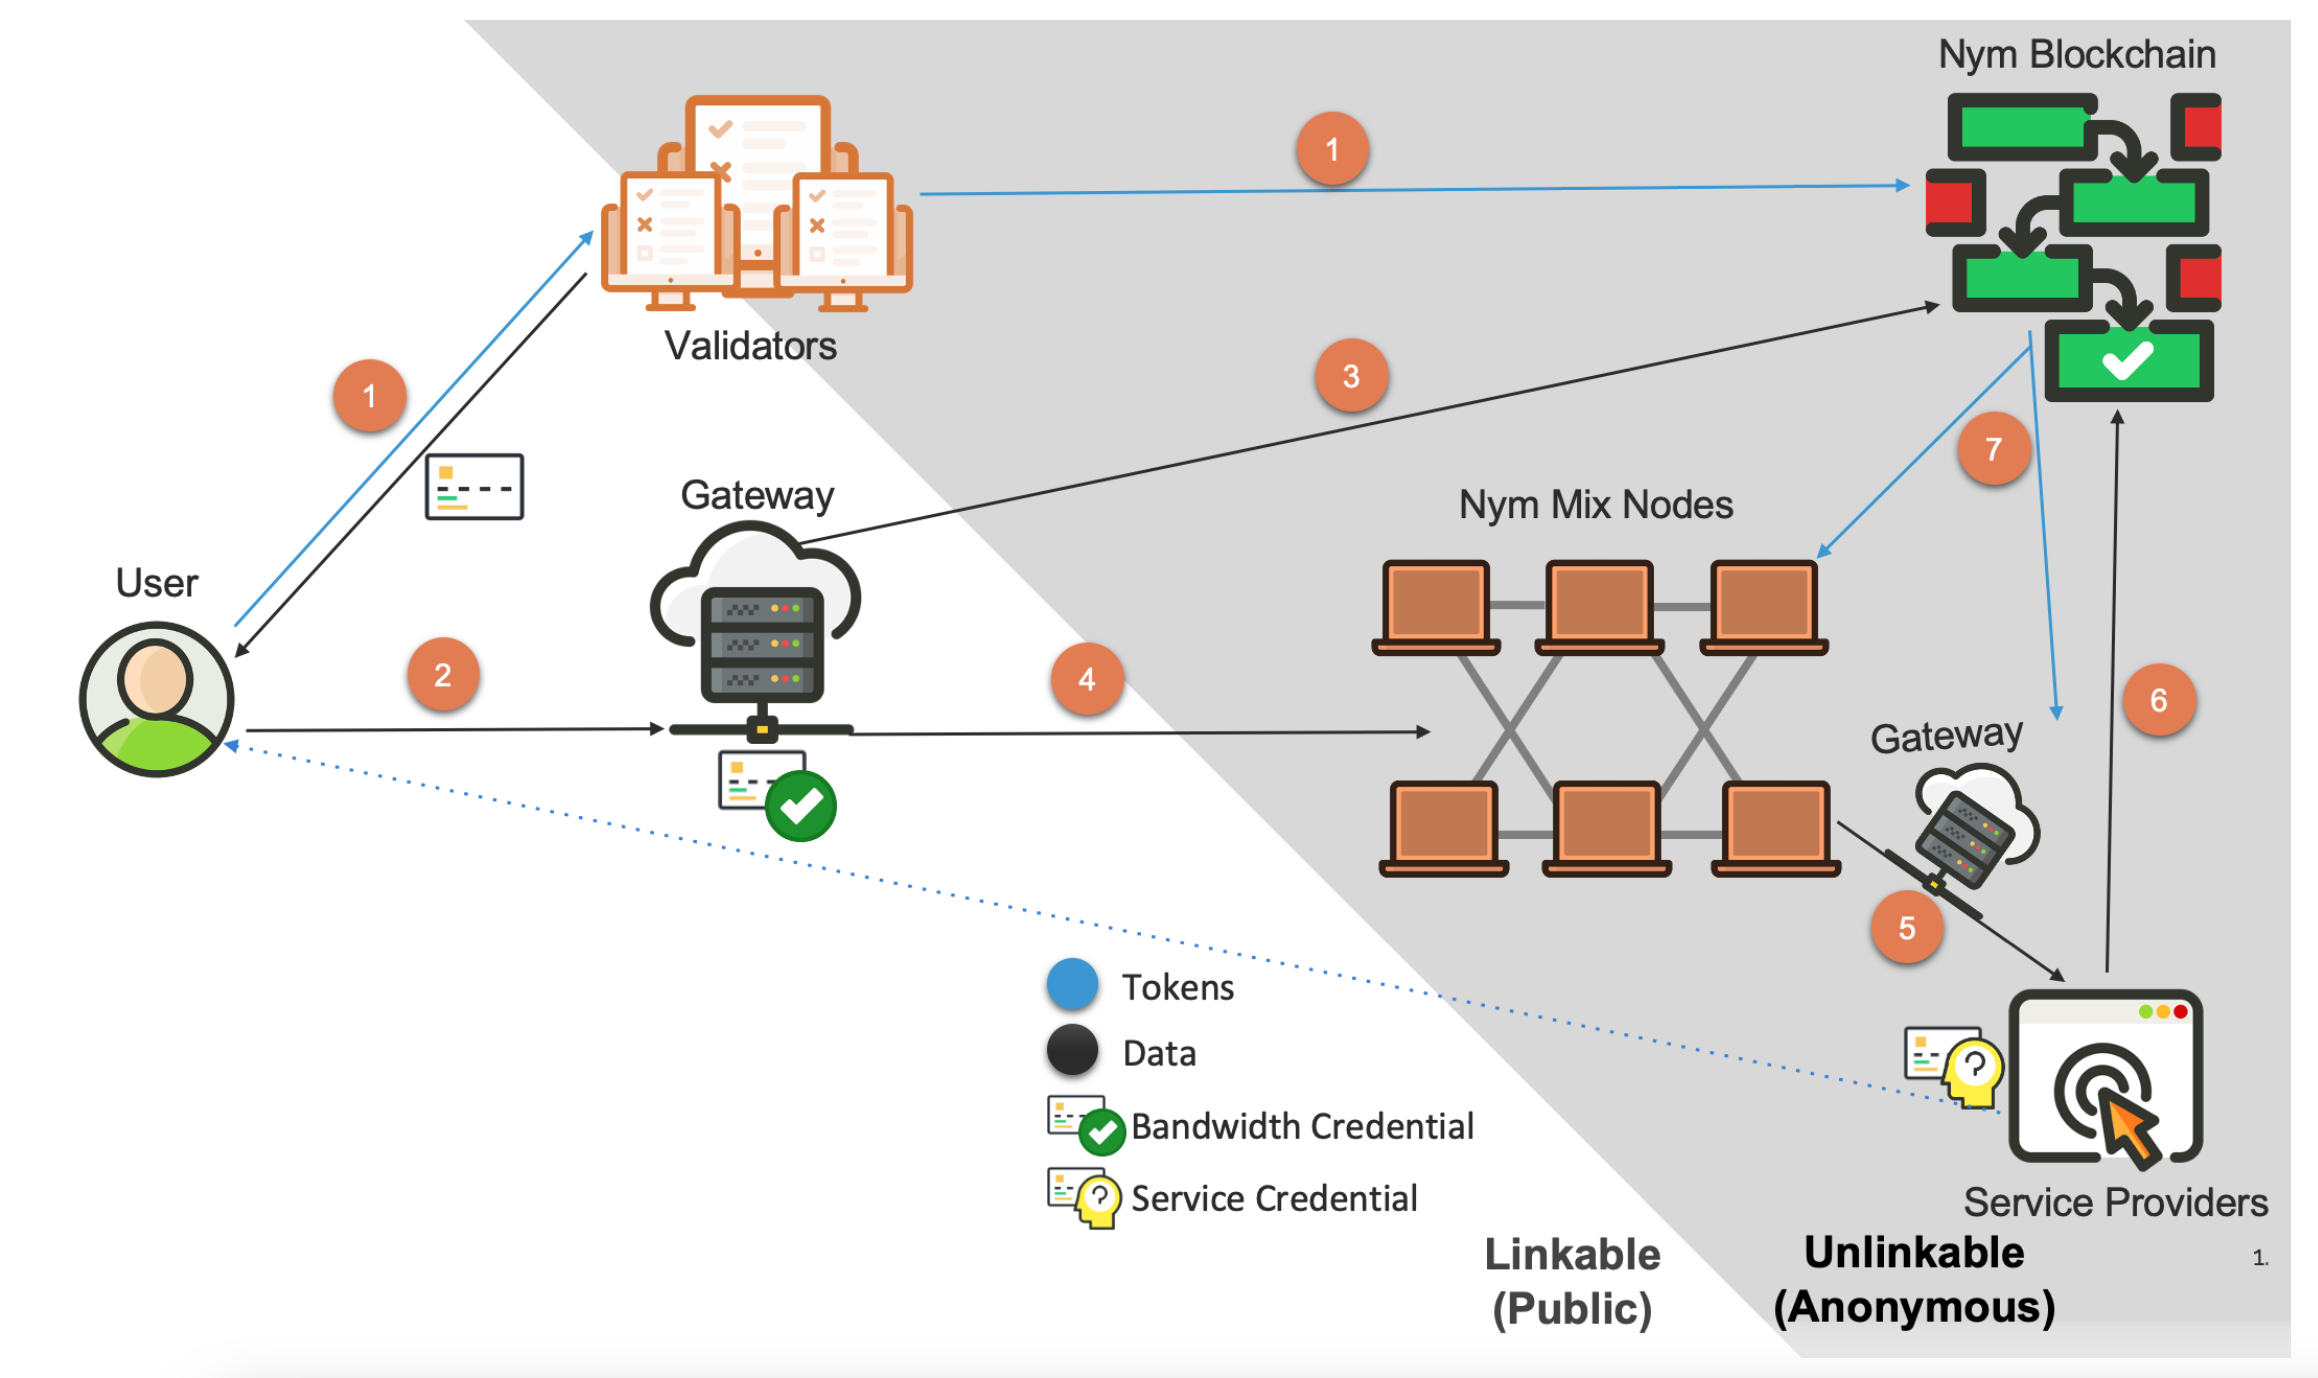
\includegraphics[width=1\textwidth]{image1.png} %1.png是图片文件的相对路径
\caption{Nym 架构和流程} %caption是图片的标题
\label{图 1} %此处的label相当于一个图片的专属标志,目的是方便上下文的引用
\end{figure}
	
	\subsection{Nym 网络参与者}
	
	Nym 网络的参与者如图 1 所示。Nym 基础设施由三种类型的节点组成:\textbf{验证器}、\textbf{网关}和\textbf{混合节点},本节接下来介绍其功能。第三方服务提供商可以通过 Nym 使自己能被访问,从而为\textbf{终端用户}提供增强的隐私。提供者还可以充当 Nym 网络和外部组件之间的接口,并且这不需要修改,甚至不需要对 Nym 的感知。例如,Nym 可用于通过服务提供商匿名广播比特币交易,该服务提供商将通过 Nym 混合网络接收到的交易中继到比特币的点对点网络。\newline

	\textbf{终端用户。}Nym的用户群包括通过 Nym 提供所有服务的用户,他们选择隐私通信,无论是匿名广播交易,访问信息,还是与朋友保持消息对话。用户群越大,越多样化,为所有用户提供的匿名性就越好,网络的成本效益也越高。\newline

	\textbf{混合节点。}混合节点通过不间断地中继数据包为终端用户提供通信隐私。混合节点组织在一个称为mixnet的网络中,数据包在传递给最终接收者之前会途经多个节点。混合节点接收数据包,它们(1)通过加密转换和(2)重新排序,这样无论是基于数据内容还是基于时间,都无法分辨哪个输入包对应于哪个输出。Nym mixnet 基于Loopix设计\cite{ref89}:它使用Sphinx数据包格式\cite{ref29}、分层网络拓扑\cite{ref36}、连续时间混合\cite{ref66}和覆盖流量循环\cite{ref30}。第4节详细介绍了Nym mixnet,包括可靠传输、可扩展性、女巫攻击保护、公平路由、服务质量度量、激励以及实际部署所需的其他修改和扩展。\newline

	\textbf{网关。}网关使 Nym mixnet 可访问,同时保护其避免搭便车行为。参与者可以选择始终为其所有流量使用相同的网关,或将流量分配到多个网关,或每天选择不同的网关。网关还为离线或无法访问的参与者缓存接收到的消息,并有助于实现可靠的传输功能。在 4.2 节中有对网关的详细描述。\newline

	\textbf{验证器。}验证器在 Nym 网络中协作执行几个核心功能。他们维护 \textbf{Nym 区块链},该区块链充当分发网络范围信息的安全广播通道,例如:活动节点及其公钥列表、网络配置参数、定期随机信标、参与者的质押、存入 \textbf{nympool}(用于支持 Nym 网络的共享资金池,下面会详细描述)、从 nympool 分发的奖励,以及需要提供给所有参与者的任何其他数据,以确保网络的安全运行。此外,验证器以分布式方式向参与者颁发凭证。\textbf{带宽凭证}对 nympool 中的存款证明进行编码,以换取通过 Nym 混合网发送的数据限额。这些凭证将向网关出示,以证明通过 mixnet 发送流量的权利。\textbf{服务凭证}可以对证明"访问"服务所需的任意属性进行编码,包括已在 nympool 中存入资金以支付服务费用的证明。\newline

	\textbf{服务供应商。}Nym 网络不是独立的服务;它是一种基础设施,支持通过它访问的广泛第三方应用程序和服务的隐私。 服务提供商可以通过 Nym 网络发送和接收消息,与他们的用户进行秘密通信,也可以选择使用 Nym 服务凭证来授予对其服务的付费访问权限,而无需进行侵犯隐私的用户身份验证。\newline
	
	\subsection{信息流}

	图 1 描述了 Nym 用户隐蔽地访问和证明他们的服务“使用权利”所遵循的步骤。数据流用黑色表示,NYM流用蓝色表示。\newline

	\textbf{(1)将资金存入 nympool 以获得凭证。}考虑已获得 NYM的用户,无论是通过购买、从服务提供商处捆绑为服务包的一部分,还是通过操作节点或与 Nym 集成的服务作为奖励获得。用户首先在 nympool 中存入代币,nympool 是由 Nym 验证器管理的共享资金池,用于支持 Nym 网络。 在此示例中,用户将其存款的一部分转换为带宽凭证,其余转换为服务凭证。用户在 nympool 中生成两个未签名的凭证以及正确性证明和存款证明,并将它们提交给 Nym 验证器。 如果一切正确,验证者就会以去中心化的方式在凭证上发出部分签名。用户收集阈值数量的部分签名以组合成有效凭证。\newline

	对存款证明进行编码的服务凭证简单地嵌入了它们所代表的代币数量以及可赎回的代币数量,而不管代币价值如何波动。另一方面,在带宽凭证的情况下,代币存款被转换为允许通过 mixnet 发送数据包的数量。 NYM和获得的带宽量之间的汇率以拍卖的形式在链上确定。为了加入网络,各个混合节点运营商提交“每包价格”函数作为其节点信息的一部分。汇率的计算考虑了当前时间窗口中作为网络一部分的节点集的每包价格函数的中值(参见第 6.3 节)。Nym 区块链用于序列化带宽凭证获取请求,使验证者能够使用每个数据包的中值函数来处理和准确定价每个请求。请注意,每个带宽凭证可以包含较大的数据包发送限额,因此,凭证操作会比通过网络发送的数据包数量少几个数量级。\newline

	\textbf{(2)使用带宽凭证访问网关。}用户根据自己的个人标准选择网关,并根据他们的存款使用带宽凭证证明他们“有权使用”Nym mixnet。网关检查带宽凭证的有效性并验证所有相关证明。\newline

	\textbf{(3)与网关建立临时Nym。}网关检查用户提交的带宽凭证是否尚未在 Nym 区块链中标记为“已花费”。然后,它向验证器提交对他们在区块链中发布的凭证中编码的序列号的承诺。此承诺将带宽凭证标记为“已使用”,并防止其在未来发生重复支出。它还允许网关证明他们路由的流量份额,以便他们可以获得成比例的奖励。用户和网关建立一个共享秘密和一个 Nym(即临时假名),与由凭证表示的数据许可和有效期相关联。用户和网关之间交换的数据使用共享秘密进行加密,网关使用 Nym 来跟踪用户消耗的数据限额。此外,用户可以将Nym用作临时邮箱地址,在那里它可以接收网关缓存的下行数据。\newline

	\textbf{(4)通过 mixnet 路由流量。}在带宽凭证的数据限额被消耗或过期之前,用户可以通过网关将流量发送到 Nym mixnet。 mixnet 匿名路由用户消息,在每一步都使输入无法链接到输出。如图 1 中白色和阴影背景区域所示,这隐藏了哪个用户正在访问哪个服务或进行哪个交易。最后一个混合节点将消息发送到接收方的网关,最终接收方从网关中提取消息。接收者可能是服务提供者、验证器或其他用户。\newline

	\textbf{(5)使用服务凭证证明“有权使用”服务。}如果被访问的提供者是接受 Nym 服务凭证作为支付证明的付费服务,则用户继续使用他们的服务凭证通过 mixnet 获得访问权限。为此,他们执行凭证显示协议,其中用户在发送给提供者的消息中包含凭证有效的证明,它嵌入了访问服务所需的正确金额,并且尚未花费。 Nym 凭证的隐私特征包括颁发和使用的凭证之间的不可链接性,再次对应于图 1 中的白色和阴影区域,使得无法从凭证显示中识别用户。\newline

	\textbf{(6)将收到的凭证标记为已使用。}接收服务凭证的提供者向区块链提交对其中编码的序列号的承诺。 此承诺是公开可用的,以防止双重支出并使提供商能够兑换凭证中编码的金额的奖励。\newline

	\textbf{(7)分配来自 nympool 的奖励。}每隔一段时间,验证器会通过算法从 nympool 中分配奖励。 这包括针对节点(混合节点、网关和验证器)维护核心 Nym 网络的工作的奖励,以及对兑换从用户处收到的服务凭证以换取服务的服务提供商的奖励。\newline
	
	\subsection{代币流}

	在 Nym 中,混合节点、网关和验证器提供网络运行需要的功能,他们因诚实的工作而获得奖励。要成为节点运营商,参与者需要质押 NYM,其中一部分可以由其他利益相关者委托。在 Nym 中,权益用作衡量节点声誉和防止女巫攻击的一种措施。在女巫攻击中,对手可以廉价地引入无限数量的节点。委托允许利益相关者通过他们的质押来支持候选节点运营商。 Nym 节点通过奖励以激励节点提供高质量的服务 (QoS),这是通过一种新颖的“proof of mixing”方案以公平和去中心化的方式衡量的。有关质押、节点选择和 QoS 测量的详细信息在第 6.2 节中进行解释。\newline

	虽然 Nym 网络节点为网络运行贡献了他们的工作和资源,但受益者是与 Nym 及其终端用户集成的第三方服务提供商。这些参与者需要带宽凭证才能通过 Nym 发送数据,发行带宽凭证所获得的收益以 NYM的形式分配给节点作为奖励。此外,Nym 服务凭证可以对可用于访问付费服务的可赎回付款证明进行编码。在这种情况下,将对用户的存款收取费用,并将剩余金额嵌入凭证中。与为获得带宽凭证而进行的存款类似,费用用于奖励 Nym 网络中的节点集。嵌入在服务凭证中的可赎回数量的代币被授予与用户一起使用凭证的服务提供商。因此,任何通过作为混合节点或验证器提供服务来使 Nym 网络正常运行的用户都会因其工作而获得 NYM 奖励。\newline

	\subsection{威胁模型}

	Nym的设计目的是在面对对手的情况下,提供比VPNs、Tor和现有点对点系统更强大的隐私。Nym 考虑的威胁模型是具有以下能力的任意组合的对手:
	
\begin{itemize}
\item \textbf{全球网络监控:}全球网络中的所有参与者和组件之间的通信,甚至互联网上的所有通信,都可以监控。此外,活跃的网络对手能够在数据包通过底层互联网基础设施传输时注入、修改和丢弃数据包。这符合大型民族国家和运营互联网基础设施的电信提供商的能力。
\item \textbf{腐败的参与者:}对手可以破坏 Nym 参与者的一个子集并协调对抗性资源来进行攻击。可能是恶意的参与者包括验证器、混合节点、网关、服务提供商和终端用户。我们假设对手用于攻击的预算(权益)有限,该预算限制了对手能够在网络中引入的对抗实体的数量。
\end{itemize}

	对抗性目标可能涉及攻击:
	
\begin{itemize}
\item \textbf{隐私:}了解 Nym 保护的隐私信息,例如:匿名广播消息的发送者;通过 Nym 访问服务的匿名用户的身份;在消息应用程序中聊天的用户之间社交关系图;属于同一用户的凭证或交易的链接(集群)。
\item \textbf{完整性和真实性:}通过以下方式违反服务完整性保证:冒充其他参与者;伪造或重播凭证(搭便车、双花);扰乱混合网络拓扑中节点的放置;扰乱网络的测量;扰乱奖励的分配。
\item \textbf{可用性:}破坏 Nym 网络的可用性,使用户无法再依赖其保护来访问服务,而是被迫以损害其隐私的方式进行通信。
\end{itemize}

	Nym 网络采用最先进的安全和隐私技术设计,以最大限度地抵御攻击,考虑到必须在整个系统中对抗对手,包括 mixnet、测量组件、支付和凭证协议。我们期望设计不断发展以包含新功能并对抗更复杂的攻击。\newline

	\subsection{隐私功能}

	Nym 网络是一种基础设施,可提供对应用程序的隐私增强访问。在这里,我们介绍 Nym 旨在实现的隐私概念。 请注意,随着网络规模的扩大,Nym 提供了更好的隐私。与每个单独的应用程序可以为其用户群提供的保护相比,通过 Nym 访问的更多用户和服务使其对所有应用程序的所有用户的隐私保护更加强大。\newline

	\textbf{不可链接性和匿名性。}在抽象意义上,\textbf{不可链接性}是指无法确定系统不同部分可用的哪些数据可能彼此相关,也可能不相关\cite{ref87}。更具体地说,考虑客户端的用户身份(例如,IP 地址、公钥、设备标识符)和服务端的消息、访问或交易。这在图 1 中以白色和阴影背景进行了说明。用户身份和服务访问之间的不可链接性相当于那些访问是\textbf{匿名的}。从服务提供者的角度来看,无法确定进行特定交易的用户是谁;在观察客户端的同时,不会泄露用户正在访问哪些服务或与谁进行通信。在某些情况下,发件人和收件人希望在实现\textbf{第三方匿名}的同时识别彼此,这意味着他们希望确保他们正在与预期的一方进行交互,同时不希望任何其他外部方能够确定他们在进行相互交流。\newline

	\textbf{匿名集。}在任何匿名系统中,提供给用户及其交易的匿名总是必然与“匿名集”相关\cite{ref87}。匿名集是从对手的角度来看可能与感兴趣的消息或交易相关联的主体集。当这个集合更大和更多样化时,交易更加匿名。同时,如果集合中的少数个人比其他人更有可能成为与交易相关的实际主体,那么交易的匿名性就会降低\cite{ref38, ref94}。组装大型和多样化匿名集的重要性使 Nym 网络具备独特的能力,可以为强大的对手提供高水平的隐私。Nym 是一个匿名覆盖网络,可以为许多应用程序路由通信,从而将所有这些应用程序的用户群融合到一个大型匿名集合中。这种级别的隐私是单一用途的独立应用程序无法实现的,只能由通用的多用途基础设施(例如 Nym)提供,该基础设施可为许多应用程序聚合用户流量。\newline

	\textbf{不可观察性}是比不可链接性和匿名性更强大的隐私功能。对于匿名性,当用户发送消息时,对手无法识别哪个输出消息对应于用户,而不可观察性意味着对手甚至无法确定用户是否正在发送任何消息。不可观察性隐藏了用户的活动模式,并将空闲用户添加到匿名集中。不可观察性是通过使用“覆盖”(或“虚假”)流量来实现的,如第 4.6 节所述。\newline

	\subsection{要求}

	除了以不可链接和匿名的形式提供隐私功能外,Nym 网络旨在满足以下要求:\newline

	\textbf{通用的。}Nym 网络是一种通用通信基础设施,可以轻松地与任何希望从其隐私功能中受益的联网应用程序集成。\newline

	\textbf{可扩展的。}Nym 网络可扩展以支持具有大量用户群的广泛服务。 Nym 使用的架构可以动态添加更多混合节点,以满足对路由隐私增强流量的日益增长的需求。此外,Nym 提供的隐私随着网络的发展而增加,集成更多的应用程序导致在匿名集中融合更多的用户。\newline

	\textbf{激励的。}为了保证高价值应用程序可以依赖 Nym 网络进行通信,Nym 通过代币化奖励来激励验证器、网关和混合节点,以确保专业维护、足够的性能和高质量的服务。激励措施旨在确保长期的诚实合作行为符合所有网络参与者的最佳利益。\newline

	\textbf{去中心化的。}Nym 网络中没有可信方、中心化组件或任何功能的单点故障,包括:路由通信、公钥发现、颁发和验证凭证、执行服务质量测量以及分配奖励。\newline

	\textbf{非许可的。}任何人都可以成为 Nym 网络中的验证器、网关或混合节点,前提是他们能够以足够的服务质量为网络贡献容量。参与者需要质押 NYM 才能成为 Nym 网络的一部分,但会根据执行有用的工作获得奖励。\newline

	\textbf{安全的。}Nym 网络采用最先进的安全和隐私技术设计,以最大限度地抵御攻击。因此,即使面对能够监控整个互联网的流量并威胁到部分Nym网络参与者的强大对手,它也可以为用户和服务提供支持。\newline
	
	\section{用于网络层隐私的 Mixnet}

	Mixnet 是一个混合节点网络,它们是转换和重新排序消息的覆盖路由器,因此它们的输入不能与其输出相关联,无论是根据消息外观、时间还是其他元数据\cite{ref25}。Nym mixnet 基于 Loopix \cite{ref89},进行了各种修改和扩展以满足第 3.6 节中概述的要求。本节概述了 Nym mixnet 架构、核心机制、设计原则和属性。\newline

	\textbf{简而言之。}Nym mixnet 的结构是混合节点层,这是第 4.1 节中证明的设计选择。Nym 使用 \emph{source-routed} 解密混合网络,用户从 Nym 区块链获取节点的公钥和联系信息。在源路由中,消息的发送者选择消息在到达其最终目的地之前要经过的路由。这个选择是根据 mixnet 的公共参数和路由策略做出的,它将混合节点分配到 mixnet 层,并根据节点容量在一个层的节点之间分配流量。\newline

	第 4.2 节介绍了网关,网关是将用户和服务连接到 mixnet 的节点。即使用户间歇性离线,网关也允许以更高的可靠性和可访问性发送和接收消息。\newline

	正如第 4.3 节中进一步描述的,Nym 使用 Sphinx \cite{ref29}数据包格式来封装和匿名路由数据有效载荷。发件人通过以反向路由顺序对它们进行多次加密来准备 Sphinx 消息。首先,为收件人加密消息;然后,对于路径中的最后一个混合节点;再然后,对于它在路径中的前一个节点,以最外层的加密结束,它对应于第一层中的混合节点。完整的 Sphinx 数据包最终使用与网关共享的密钥加密,网关将解密的 Sphinx 数据包转发到 mixnet。\newline

	当混合节点收到一条 Sphinx 消息时,它会使用自己的私钥剥离一层加密,检索将消息路由到下一跳的信息,并对消息进行加密转换,使其无法识别。在将消息转发到消息路由中的下一个节点之前,混合节点还会将消息保留一段随机时间,如第 4.4 节所述。可以使用“single use reply blocks”(SURBs) 发送对消息的响应,详见第 4.5 节。\newline

	Nym mixnet 生成覆盖流量“循环”,如第 4.6 节所述。 混合节点生成的循环始终确保最低级别的匿名性,而终端用户可以生成循环来混淆他们通过 Nym 的进行通信的时间和数量,从而实现不可观察性。\newline

	如第 4.7 节所述,混合节点成员资格以及混合网络的大小和参数在每个 epoch 的基础上定期更新。随着通过 Nym 可以访问更多服务,这使得网络能够发展和扩展,以充分满足所有用户的需求。\newline

	最后,在第 4.8 节中,我们讨论了在设置 mixnet 参数时必须考虑的延迟、带宽和隐私之间的权衡。我们还解释了隐私和可扩展性之间的正相关:随着使用量的增加,可以添加新的混合节点以(线性)增加容量,隐私可以保持在较高水平,同时允许更低的延迟和覆盖流量开销。\newline

	\textbf{与洋葱路由的比较。}“覆盖代理路由器”、“源路由”和“分层加密”也是洋葱路由的特点。尽管 mixnet 和洋葱路由网络(如 Tor)之间有相似之处,但这两种类型的系统之间也存在重要差异:
	
\begin{enumerate}[1. ]
\item 虽然洋葱路由创建了在会话期间承载与电路相关的所有数据包的电路,但混合网络通过不同的路由独立路由每条消息,并且不保证按顺序传递。这使得跟踪端到端数据流变得更加困难,即使对于监控网络中所有连接的对手也是如此。
\item 洋葱路由器以先进先出的顺序沿电路转发数据包,而不会改变流量的时间特性。相比之下,混合节点不仅可以进行密码转换,还可以延迟和重新排序消息,从而防止基于时间信息将输入链接到输出消息的攻击。
\item 虽然洋葱路由系统通常不使用任何覆盖流量,但 Nym mix 网络会生成覆盖流量循环,以始终保证足够的匿名性。此外,覆盖流量为客户端提供了不可观察性,以至于根本无法确定用户是否正在进行通信。
\end{enumerate}

\begin{figure}
\centering
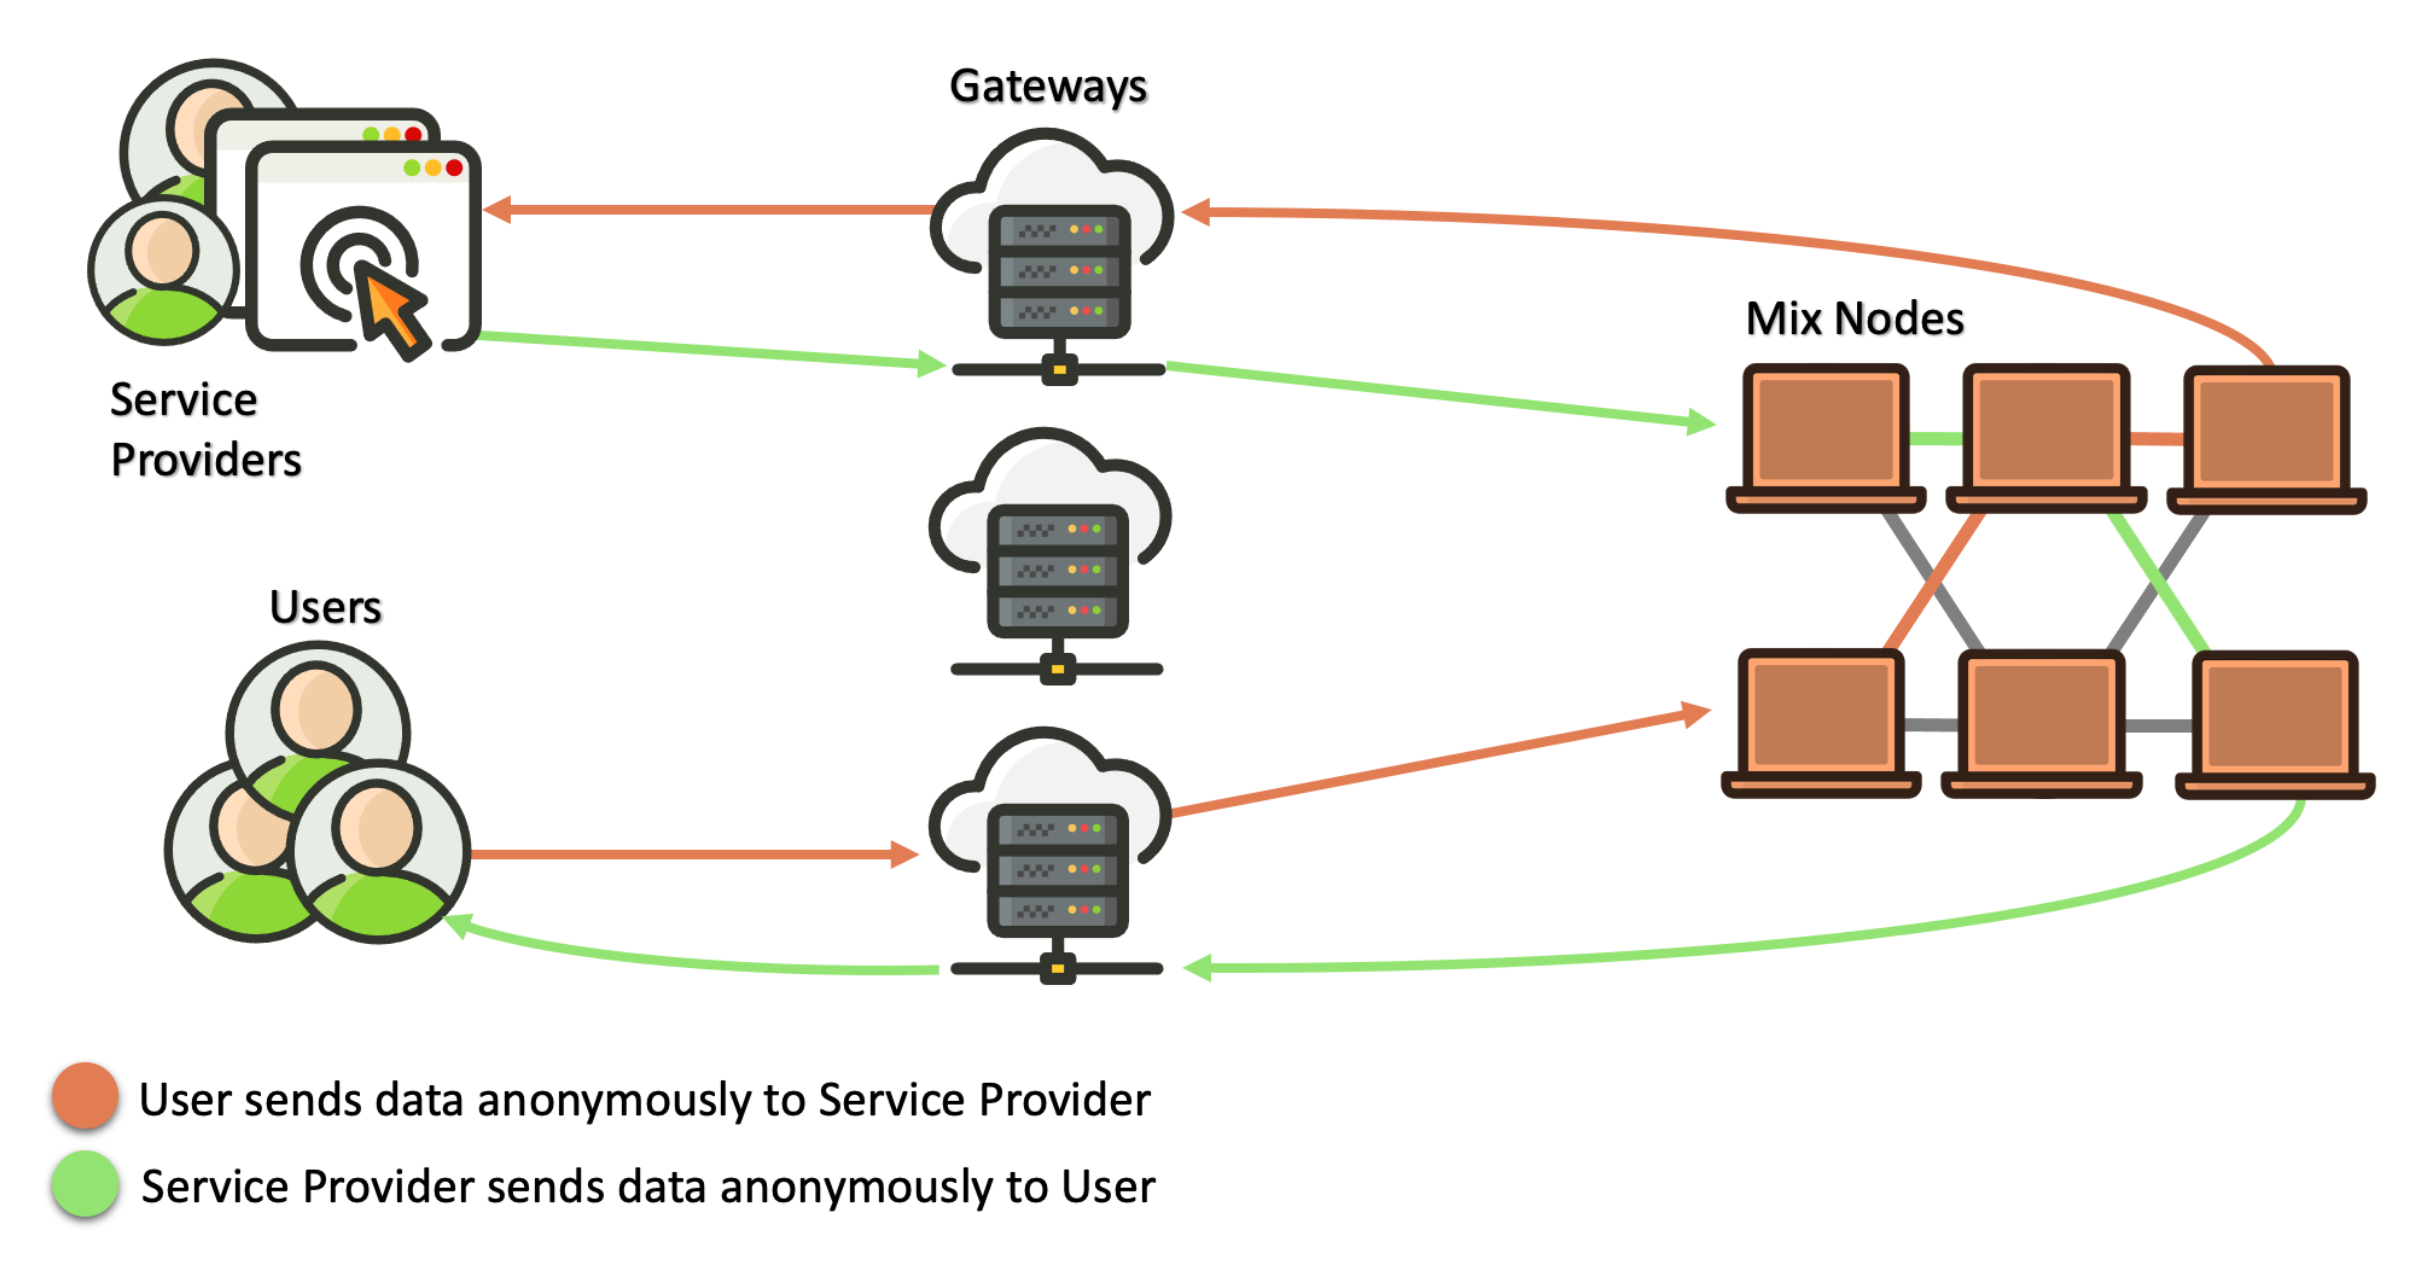
\includegraphics[width=1\textwidth]{image2.png} %1.png是图片文件的相对路径
\caption{用户和服务通过网关和具有 3 层节点的 mixnet 进行隐私通信} %caption是图片的标题
\label{图 2} %此处的label相当于一个图片的专属标志,目的是方便上下文的引用
\end{figure}

	\subsection{分层混合网络拓扑}
	
	Nym mixnet 具有分层网络拓扑结构,其中混合节点按层排列,如图 2 所示。该拓扑结构已显示出对于隐私、可扩展性和易于分析的最佳选择\cite{ref7, ref36}。特别是,分层混合网络通过简单地向现有层添加混合节点来扩展以处理更多流量,而隐私可以通过添加层来增加。\newline

	考虑到足够多的候选混合节点,定期选择一个子集在网络中活跃地运行。选择概率与节点的权益成正比,如第 6.3 节所述,它充当节点声誉的指标。未选择的节点将保留到下一个 epoch 。一旦确定了下一个时间段的成员资格,节点到层的分配就会随机化,以防止节点的恶意联盟战略性地优化它们在网络中的位置以促进攻击。为了避免依赖集中的可信方,Nym 将混合节点分配到层的算法是去中心化的且可公开验证的。该算法利用可验证随机函数(VRF)\cite{ref80},该函数在每个 epoch 之前运行。每个混合节点 $i$ 都有一个公钥对 $\left ( pk_{i}, sk_{i} \right )$,在它们的节点描述符中公开可用。在一个epoch开始之前,验证者在 Nym 区块链中共同发布一个随机信标 $x$ 。混合节点结合他们自己的私钥 $sk_{i}$ 计算与输入 $x$ 相对应的 VRF 输出 $y_{i}$ 和相关证明 $\pi_{i}$,即 $y_{i},\pi_{i}\leftarrow VRF(x,sk_{i})$。考虑三个 mixnet 层,epoch 节点的层计算为:$y_{i} \mod 3$,将其推广到任意数量的 L 层为:$y_{i} \mod L$。混合节点向验证器广播 $(y_{i}, \pi_{i})$,验证器在 Nym 区块链中公开该值。所有参与者都可以使用 $\pi_{i}$ 来验证 $y_{i}$ 是否正确,并重建哪些节点属于 mixnet 的哪一层。请注意,当参与者注册为网络中的候选运营商时,节点的公钥是提前发布的。那时节点不可能预测哪个公钥会导致在接下来的 epoch 中的特定网络位置。\newline

	分层路由意味着第一层混合节点仅接收来自网关的消息,而后续层的节点仅接收来自前一层节点的消息。类似地,网关和混合节点仅将消息中继到后续层中的节点。最终接收者可能是验证器、服务提供商或在其设备中运行 Nym 客户端的任何参与者。为了平衡网络中的流量负载,路由算法在每一层内选择一个节点,并根据节点的容量加权概率。最小和最大容量限制确保所有混合节点对网络运营做出有意义的贡献,而没有混合节点路由不成比例的大部分流量。\newline

	分层路由和混合节点到层的随机分配使控制节点子集的攻击者难以破坏大部分消息。考虑到一个具有 L 层的网络,攻击者需要控制每一层中的一个节点,以完全消除消息的匿名性——如果攻击者甚至无法填充一层,那么任何消息都将无法端到端地追踪。对于对手来说,最好的情况是当对抗节点均匀分布在所有层时,因为这可以最大限度地减少可能受到威胁的端到端路由的比例。即使在最好的容量占比 $\alpha$ ,端到端可追踪路由的占比由 $\alpha^L$ 给出。因此,在 $L = 3$ 层的网络中,控制 50\% 混合节点 $(\alpha = 0.5)$ 的对手将能够观察到最有利拓扑配置中 12.5\% 的消息,而控制 10\% 混合节点的对手将能够观察到每层中的节点 $(\alpha = 0.1)$ 只会完全观察 0.1\% 的消息。如果层数增加到 $L = 4$,那么控制 50\% 节点的对手在最好的情况下会观察到 6\% 的消息,而控制 10\% 的对手只会看到 0.01\%。\newline

	\subsection{网关}

	网关促成对 Nym 网络的访问。它们是位于 mixnet 和发送/接收消息的参与者之间的代理,如图 2 所示。如第 5 节所述,参与者必须向他们选择的网关出示有效的未使用带宽凭证,才能使数据通过Nym 混合网络。网关通过收集带宽凭证并将流量限制为凭证限额来保护 mixnet 免受搭便车者的侵害。网关也使用这些凭证来证明它们所服务的流量并要求相应的奖励。在显示有效的带宽凭证后,发送方和网关建立一个共享秘密,该秘密在带宽凭证的数据限额被消耗或过期之前一直有效。从共享密钥派生的密钥用于对称加密发送方和网关之间的流量。网关不执行 Sphinx 处理或混合,因此他们可以非常有效地将消息转发到 mixnet。\newline

	参与者可以自由地为他们的所有消息使用一个网关,或者在多个网关之间分配他们的流量。在后一种情况下,他们为每个网关使用单独的带宽凭证。请注意,从网络的角度来看,参与者对网关不是匿名的,因为网关可以看到连接到他们的参与者的 IP 地址。然而,网关没有关于其消息目的地的信息,甚至没有关于消息是否携带任何真实数据的信息。网关还为其用户接收和存储消息,用户可以指定他们的临时假名作为接收消息的返回地址。这样,即使用户不总是在线,也能够可靠地接收消息。\newline

	网关不会延迟或重新排序消息,因此不会提供 mixnet 的不可链接属性。相反,网关能够通过提供抗审查能力来促进世界各地的参与者访问 Nym 网络。某些位置的用户甚至可能需要伪装他们对 Nym 网络的使用,以便本地攻击者根本无法检测到用户是否通过 Nym 发送互联网流量。网关可以使用协议将进入 Nym 网络的第一“跳”伪装成其他类型的流量,从而使这成为可能。\newline

	网关必须注册一个描述符,包括它们的公钥、网络地址(IP、端口)、容量和已提交权益的证明,就像所有 Nym 节点一样。请注意,网关的网络地址对于仅接受来自属于 Nym 网络一部分网关的消息的第一层混合节点和仅向有效网关发送消息的最后一层混合节点很重要。对于终端用户,网关可以提供许多不同的面向用户的网络地址和通过不同渠道宣传的连接协议。否则,通过简单地将公开可用的网关 IP 地址列表列入黑名单来审查对 Nym 网络的访问将是微不足道的。 Nym 允许多种网关实现、配置和审查规避策略,以便为终端用户提供多种方式来连接到 Nym 网络而不会被检测或审查。用户和网关之间的接口将建立在类似于为 Tor 的可插拔传输提出的那些概念的基础上,以使用户能够在受到高度审查的地区进行访问\cite{ref11, ref81}。网关还可以使用 VPN 协议(从 OpenVPN 等标准到 Wireguard 等更新的协议)与用户进行通信。\newline

	\subsection{Sphinx 数据包格式}

	Nym 使用 Sphinx 数据包格式对应用程序的有效负载数据进行编码\cite{ref29}。Sphinx 是一种紧凑而高效的加密数据包格式,最初设计用于为混合网络中的多跳路由提供按位不可链接性。对于数十 KB 的有效载荷大小,Sphinx 标头引入的开销约为 1\%——几百个额外字节。\newline
	
\begin{figure}
\centering
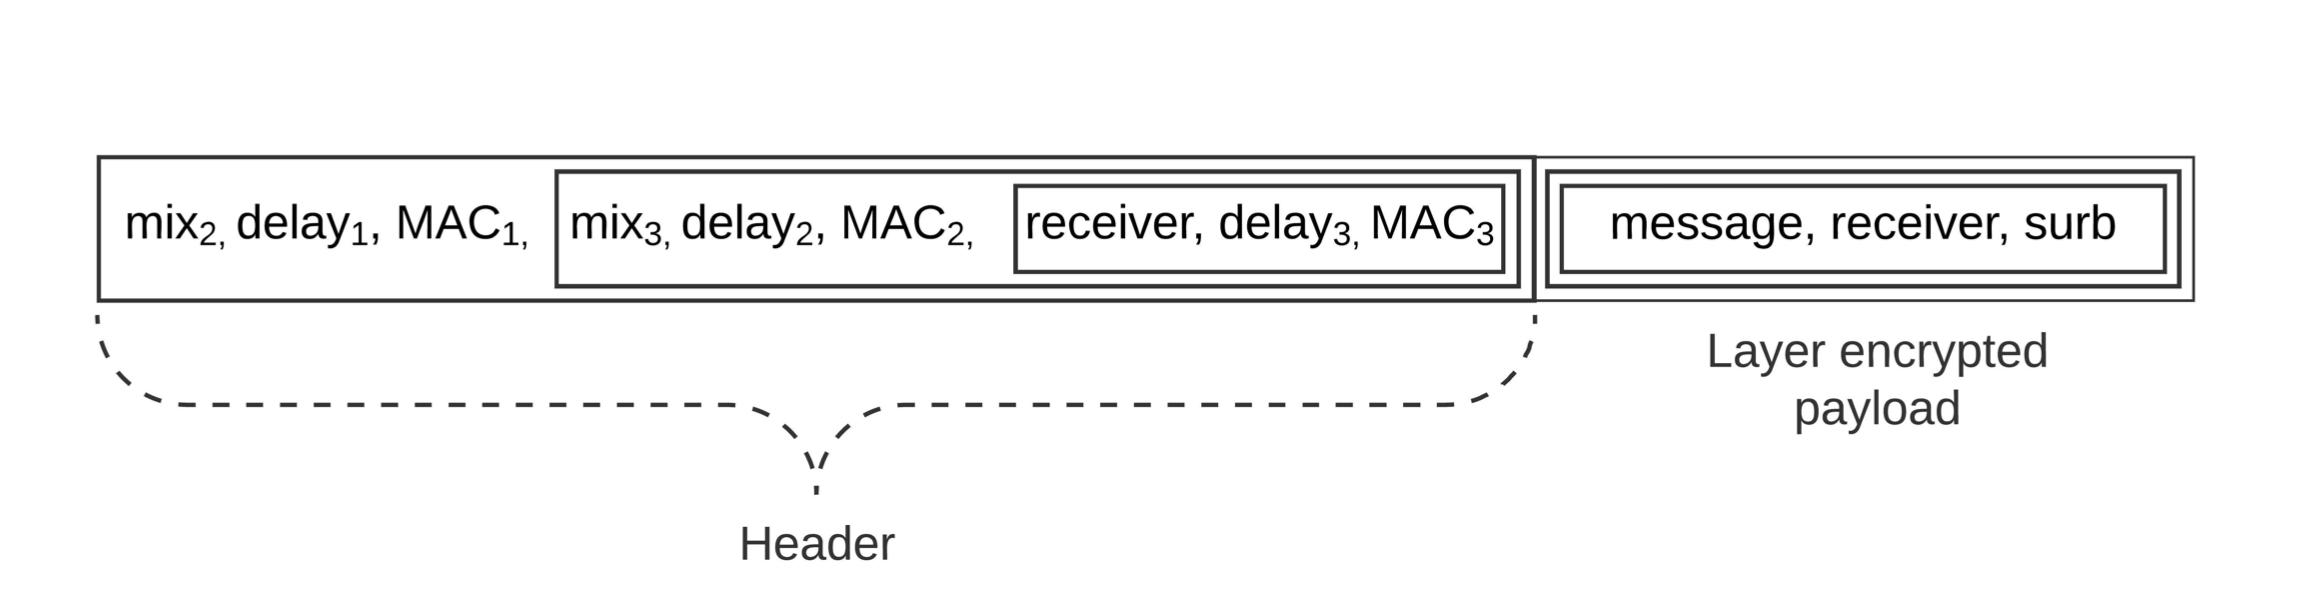
\includegraphics[width=1\textwidth]{image3.png} %1.png是图片文件的相对路径
\caption{Sphinx包格式} %caption是图片的标题
\label{图 3} %此处的label相当于一个图片的专属标志,目的是方便上下文的引用
\end{figure}

	Sphinx 允许在层中加密消息并通过多跳路由它们,这样消息头和有效负载在每跳上都是加密不可链接的。要创建 Sphinx 消息,客户端首先使用随机选择的组元素和节点的公钥与消息路由中的每个混合节点派生一个共享密钥。然后,客户端使用派生的共享密钥将消息包装在多层加密中,如图 3 所示,为消息路径中的每个节点添加消息身份验证代码和路由信息。这使每跳的报头完整性验证成为可能,同时保留消息不可链接属性,即使是在消息路由中串通对抗混合节点也是如此。Sphinx 数据包被填充为恒定长度以避免基于大小的攻击。虽然同一个 mixnet 可以支持多个数据包大小,但数据包只能与相同大小的数据包混合。\newline

	收到 Sphinx 消息后,混合节点将消息头中的循环组元素与其自己的私钥组合在一起。这使节点能够计算解密消息并验证其完整性所需的共享密钥。每跳的解密路由信息包括消息在转发之前应该延迟的时间量以及它应该发送到的下一跳的地址。作为消息处理的一部分,该节点盲化消息中的组元素,因此输出消息在密码上不可链接到输入。消息路由中的下一个节点将使用转换后的(盲)组元素来计算自己正确的共享密钥并执行自己的 Sphinx 消息处理。Sphinx 具有针对主动标记攻击的内置保护\cite{ref88},使混合节点能够检测和丢弃已被篡改的消息。混合节点还保留所见消息的组元素列表,并丢弃重复的消息以防止重放攻击。\newline

	\subsection{连续时间混合和指数延迟}

	混合节点之所以得名,是因为它们在发送消息之前“混合”了消息。但是,可以实施多种混合策略来重新排序消息。早期的混合节点提议通过 batching 和 shuffling \cite{ref16} 实现了消息重新排序。这种简单的设计会收集大量输入消息并输出这些消息的随机排列,但已知存在一些缺点:此类混合网络中消息的端到端延迟既无界也无可预测,并且由定期刷新批量消息引起的突发通信使这些混合设计在利用带宽方面效率低下。在匿名性方面,已知简单的批处理策略提供低匿名性 \cite{ref35, ref37},并且特别容易受到攻击\cite{ref26, ref31, ref95}。\newline
	
\begin{figure}
\centering
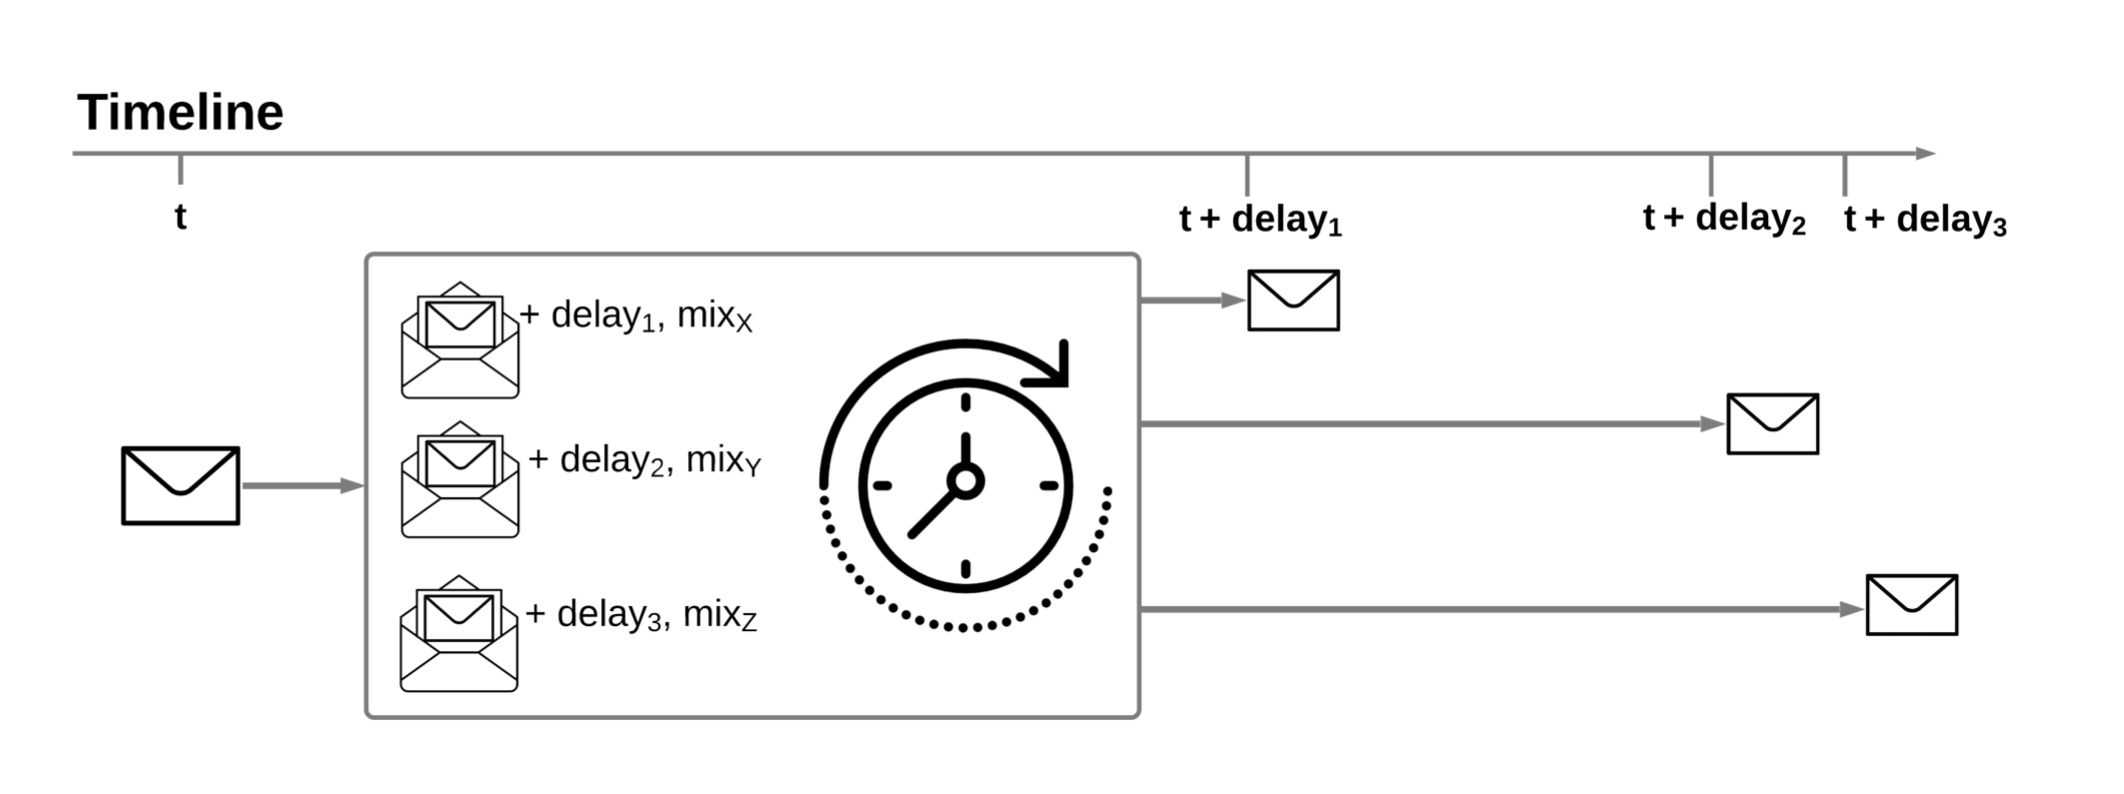
\includegraphics[width=1\textwidth]{image4.png} %1.png是图片文件的相对路径
\caption{连续时间混合} %caption是图片的标题
\label{图 4} %此处的label相当于一个图片的专属标志,目的是方便上下文的引用
\end{figure}

	与 Loopix \cite{ref89} 类似,Nym 使用连续时间混合节点 \cite{ref66} 。连续时间混合策略,如图 4 所示,独立延迟每条消息,一旦指定的延迟超时,就将其转发到下一个目的地。独立延迟每条消息的聚合效果是一个输出消息序列,该序列相对于输入序列随机重新排序。已知具有指数选择延迟的连续时间混合可为给定的平均端到端延迟提供最佳匿名属性 \cite{ref24},这是因为指数分布的无记忆特性。这个属性意味着,如果我们观察到两条消息在时间 $t_{0} < t_{1}$ 进入混合节点,并且一条消息在稍后时间 $t_{2}$ 出来,那么输出是两个输入中的任何一个的概率是相等的,无论到达时间 $t_{0}$ 和 $t_{1}$的差异如何。\newline

	与 Elixxir \cite{ref19} XRD \cite{ref70} 和 Vuvuzela \cite{ref103} 中使用的批处理混合相比,它们产生有限的匿名集,连续时间混合具有更大的(理论上无界的)匿名集。这是因为指数分布是长尾分布的,即使大多数延迟很短,消息也有非零概率导致大延迟;因此,攻击者不能丢弃未来的混合输出消息作为它想要跟踪的输入的候选者(但实际上,一旦概率低于可忽略的阈值,指数分布的无限长尾就会被截断)。 此外,由于这些混合节点连续发送和接收消息,因此它们比批处理混合更有效地使用带宽。\newline

	消息在节点中停留的时间由原始发送者选择,并编码在发送到每个混合节点的 Sphinx 标头中。与批处理 mixnet 相比,这带来了连续时间混合的重要实际优势:鉴于发送方自己在路由的每一跳处生成和编码消息的延迟,他们可以预测他们的消息何时会被传递。发送方使用的指数分布的平均参数决定了预期的端到端延迟和提供给消息的匿名性之间的权衡。如果混合网络中的流量保持不变,则导致更多延迟的配置会自动提供更强的匿名性。\newline

	我们希望 Nym 生态系统中的应用程序具有从一秒(例如,对于即时消息和闪电网络支付渠道)到几分钟(例如,对于非交互式交易和文件共享应用程序)的端到端延迟容限。为了提供可以适应广泛用例的通用基础设施,在为应用程序路由流量时,Nym 客户端会考虑其延迟容限,以设置从它提取每跳延迟的位置的分布平均值。请注意,延迟分布的应用相关方差牺牲了灵活性以提高应用程序流量向中间混合节点的可区分性,因为某些(非常大或非常小的)延迟更可能与某些应用程序而不是其他应用程序相关联。另一方面,当考虑监控所有混合节点的输入和输出但无法看到消息中编码的每跳延迟的网络对手时,具有大延迟容限的应用程序为低延迟应用程序增加了保护\cite{ref43}。此外,与 XRD \cite{ref70} 和 Vuvuzela \cite{ref103} 等系统相比,Nym 支持具有不同流量负载的用例,后者假设每个用户每轮只传达一条消息。\newline

	\subsection{匿名回复和使用一次性回复块(SURBs)的可靠传输}

	缺乏可靠传输历来是 mixnet 的一个问题,如果用户无法确定他们的消息是否被传递,mixnet 的功能就会严重削弱。为了解决这个长期存在的问题并作为隐私的通用互联网基础设施,Nym 利用连续混合提供的可预测的端到端延迟,结合 Sphinx 的一个非常有用的功能:一次性使用回复块 (SURBs)。SURBs是预先计算的Sphinx数据包头,编码一个以创建SURB的参与者为终点的 mixnet 路由。发件人可以生成一个或多个 SURB,并将它们包含在发送给收件人的 Sphinx 消息中。接收者可以使用 SURBs 作为 Sphinx 标头来发回回复或确认,在通过 mixnet 后匿名返回给原始发件人。\newline

	SURBs 是 Tor 中“洋葱地址”的 Sphinx 等价物,但需要注意的是 SURB 只能使用一次(以防止重放攻击)并且在其有效 epoch 内(用于准备 SURB 的混合节点公钥仅在有限的时间内有效)。SURB 标头由发送方加密,因此将其发回的接收方无法从中推断出有关消息路由、每跳延迟或发送方地址的任何信息,这些信息在 SURB 的最内(最后)路由层中编码。请注意,回复路径中第一个混合节点的身份必须对接收者可见,因为他们必须知道向哪个节点发送回复(通过接收者自己的网关隧道)。一个 SURB 有效地包含:(1)Sphinx 消息的加密Header,如果发送到 mixnet,将被路由回原始发送者; (2) 应该发送消息的第一层混合节点的地址; (3) 用于加密回复有效载荷的加密密钥。\newline

	收到包含 SURB 的消息后,接收者可以获取数据有效负载,使用随 SURB 一起提供的加密密钥对其进行处理,将有效负载附加到 SURB 中接收的Header,然后将消息发送到适当的第一层混合节点 (通过接收方选择的网关)。Sphinx 的设计使得新(转发)消息与 SURB(回复)消息无法区分,即使是路由消息的混合节点也是如此。通过这种方式,回复和转发消息融合成一个大型匿名集,加强了 mixnet 的整体匿名属性。\newline

	除了启用匿名回复外,Nym 网络还使用 SURB 来提供可靠的传输,即使网络中出现数据包丢失也是如此。这是通过在 Sphinx 消息中包含一个 SURB 来实现的,在寻址到接收者网关的层中。网关立即将 SURB 发送回 mixnet,让匿名发件人知道消息已收到,可选地在有效负载中包含标志,例如,发出错误信号,例如“收件人未知”或“收件人邮箱已满”。SURB 寻址到接收者的网关而不是最终接收者,因为接收者可能并不总是在线,而网关是一个永远在线的服务,可以在收到消息时立即发回确认。如果在预期的时间范围内没有收到确认(转发消息和 SURB 中的每跳延迟之和以及两个方向的混合节点之间的传播时间的估计),则发送方重新传输消息。\newline

	参与者可能还希望广播 SURB 作为一种在不暴露其位置的情况下可公开访问的方式,例如,希望在不公开其 IP 地址的情况下建立支付通道的闪电网络节点,以保护托管在这些服务器中的钱包。总之,SURB 是使 Nym mixnet 成为一个隐私通信基础设施的一个功能,足以支持广泛的应用程序,远远超出电子邮件和投票这两个 mixnet 文献中的规范用例。\newline

	\subsection{通过覆盖流量循环实现不可观察性}

	就元数据保护而言,隐藏“谁向谁发送消息”是一种必要的 mixnet 属性,但这并不总是足以防止监视。随着时间的推移,观察发送和接收消息的数量和时间的对手可能仍然能够推断出隐私信息,即使个别消息是高度匿名的\cite{ref32}。关于用户交互的数量和时间的详细数据会随着时间的推移泄露关于用户访问哪些服务以及这些服务的使用模式等信息。如果用户从事持久的行为(例如,总是给同一个朋友发消息或总是访问同一个服务),通信配置文件可能会随着时间的推移而泄漏,并且可以通过长期的统计披露攻击来恢复 \cite{ref26, ref31}。Mixnets,包括经典的 Chaumian 批处理 mixnets,它们提供了不可链接性,但不提供不可观察性 \cite{ref87}。为了使对 Nym 的访问无法被观察到,攻击者不应该知道参与者何时发送或接收了多少实际流量。\newline

	覆盖流量通过添加不携带有效载荷数据并在最终目的地被简单丢弃的“虚拟”消息来伪装真实的流量模式。在路由消息时,混合节点无法区分它是虚拟消息还是承载用户数据的正常消息。最初提议将虚拟流量路由回发送方而不是在随机选择的目的地结束,以主动检测对混合网络的主动攻击 \cite{ref30}。 Loopix,其名称指的是它使用覆盖流量的“循环”,扩展了这种方法以保证终端用户的匿名性和不可观察性的下限\cite{ref89}。Nym 遵循类似的方法,参与者生成循环传播的虚拟消息,并将自己作为最终目的地。\newline

	循环消息是按照泊松过程以随机间隔生成的。它们由混合节点生成,以确保网络中随着时间的推移有足够的流量,从而保证大型匿名集和高度隐私。终端用户和服务可以选择生成循环消息来混淆他们的活动模式。当对手看到参与者发送或接收消息时,它无法区分他们是在主动通信还是只是发送和接收空的循环。在循环回发送方的路由中发送覆盖流量使用户和混合节点都能够保持有关网络健康状况的本地更新知识,包括检测节点何时出现故障、拥塞或受到攻击的能力 \cite{ref30}。\newline

	\subsection{混合网络 epoch}

	Epoch 是重新配置 Nym 混合网络的固定时间间隔。由于多种原因,这种定期重新配置是必要的。首先,需要更新混合节点解密密钥以提供前向安全性,否则混合节点可能会被强制使用其私钥来解密旧的重播消息。每个 epoch 更新密钥的另一个好处是,节点可以忘记每次 epoch 更改时看到的消息列表,因为来自先前 epoch 的重放消息无法再解密或路由,因为必要的解密密钥不再有效或可用。请注意,每次 epoch 更新仅影响混合节点解密密钥,而不影响用于身份验证的长期签名密钥。其次,定期重建 mixnet 拓扑使系统能够从出现故障或失去声誉的节点中恢复,并在需要更多容量时重新平衡层并向网络添加新的混合节点。最后,要获得准确的测量结果,需要对混合节点的性能进行采样,该混合节点放置在不同的混合网络层,具有不同的前驱和后继集,这样即使某些节点是恶意的,它们也无法始终以节点为目标来偏向其测量。\newline

	在 epoch 持续时间方面,更短的 epoch 有利于前向安全性、更好的节点性能采样以及对混合节点流失和用户需求波动的更快反应。另一方面,更短的 epoch 也会导致更多的开销,因为需要更频繁地收集节点描述符并将其分发给所有参与者,并且必须更频繁地运行用于将节点分配到层的协议。短的 epoch 也会对匿名性产生不利影响。这是因为匿名集在每个 epoch 都是不相交的:消息在不同的密钥下加密并遵循不同的网络拓扑这一事实,意味着它们不可能跨 epoch “混淆”(即混合)。虽然会有 epoch 持续时间的动态优化,但预计 epoch 将在几小时或几天的数量级。这比消息的端到端延迟大几个数量级,因此对匿名集的影响有限。预计消息不会在 mixnet 中保留数小时,因此这些未来的消息无论如何都不会做出有意义的贡献到更早输入的匿名消息集。请注意,网络必须提前为至少一个 mixnet epoch 提供可用的密钥和配置信息,以便用户能够准备在未来一段时间内有效的数据包和响应头。需要仔细设计并考虑极端情况,以确保对手无法利用 epoch 切换条件来减少某些消息的匿名性。\newline

	\subsection{延迟、带宽、可扩展性和隐私}

	匿名通信系统必须在延迟、带宽消耗和隐私属性之间进行权衡 \cite{ref33}。Nym 使用的连续时间混合节点能够支持具有不同延迟约束的应用程序,因为隐私和端到端延迟之间的权衡可以通过改变用于选择每个节点的指数分布的平均值来调整。消息中编码的跳跃延迟。另一个权衡是在覆盖流量循环消耗的带宽与此覆盖流量提供的保护之间,无论是在匿名性还是不可观察性方面。Nym 客户端可以配置为通过更改泊松参数值来生成或多或少的覆盖流量,从而调整带宽消耗和隐私之间的权衡。\newline

	可扩展性是大规模采用任何系统的关键,但这在匿名系统的情况下更为重要。因为众所周知,\emph{anonymity loves company}\cite{ref41},这意味着匿名属性的强度取决于系统中的用户数量。因此,网络级匿名系统应该扩展到数百万用户才能真正有效。Nym 使用的分层混合网络拓扑可以通过向混合网络层添加更多节点来扩展。这与 Elixxir \cite{ref16, ref19}、XRD\cite{ref70} 或 Vuvuzela \cite{ref103} 中使用的级联混合网络形成对比,其中一旦级联达到其全部容量,就需要使用新的不相交级联,随后进行分区和匿名集的大小上限。相反,在分层网络中,添加更多混合节点以增加容量和处理更多流量负载有助于提高向混合网络所有用户提供的整体匿名性,从而在可扩展性和匿名性之间产生协同作用。\newline

	此外,增加的用户和消息数量允许降低端到端延迟和覆盖流量,同时仍然提供高度的匿名性,这反过来又使 Nym mixnet 能够支持具有更严格延迟限制的应用程序。为不同的应用程序集提供服务也会影响匿名集的质量,因为攻击者无法推断出用户正在访问哪些服务(如果有的话),因此使用网络这一事实本身就非常缺乏信息。通过专注于提供灵活、可配置的隐私通信基础设施,该基础设施可以扩展并支持广泛的应用程序,Nym 网络能够为其所有用户提供大量多样的匿名集,这是任何与 Nym 集成的应用程序通过它自己都无法实现的。\newline

	Nym 具有\textbf{水平可扩展性},因为满足不断增长的需求只需添加更多混合节点。从真实用户发送的流量越多,所有用户获得的隐私就越多,在保持隐私的同时,覆盖流量甚至可以减少。\newline
	
	\section{隐蔽证明“使用权”的凭证}

	网络元数据的保护对于实施隐私增强服务是必要的,但这还不够。特别是,确定用户是否有权获得服务的机制通常依赖于涉及不必要的用户识别和跟踪的侵犯隐私的做法。正如爱德华·斯诺登 (Edward Snowden) 所说,我们需要的是保护隐私的“使用权”证明。
	
	\begin{displayquote}
	\emph{“We are gating access to the infrastructure necessary for life through this process of proving who you are rather than proving a "right to use" —\, that you paid for this, that you should be able to access this, that you have a blinded token of some type... It [shouldn't] matter who I am, I'm allowed to be here, I'm supporting the infrastructure, I've done my part, and that’s all it should be. Otherwise we’re being forced to give up ownership of our identities and our histories. We’re allowing others to control the story of our private lives.” \\ \begin{flushright}Edward Snowden, Web3 Summit, 20 August 2019\end{flushright}}
	\end{displayquote}
	
	在许多情况下,访问权限是在为服务付费后授予用户的。Zcash \cite{ref92} 或 Monero \cite{ref82} 等加密货币提供隐私支付功能,如果仅根据货币支付确定用户的使用权,则可以使用这些加密货币进行支付。然而,管理用户在服务中的使用权(也可以称为身份管理,因为权限可能取决于用户的身份属性)通常更复杂。例如,某些服务可能要求用户在授予访问权限之前出示年龄证明、居住国家/地区或 KYC/AML状态。在其他服务中,用户可能因为他们是学生、老年人或高级会员而有权享受折扣。现有的隐私保护加密货币,例如 Zcash 和 Monero,除了简单的货币支付之外,缺乏支持更广泛意义上的身份和访问权限管理的灵活性。\newline

	Nym 凭证可以对与证明使用权相关的任何属性进行编码,包括第三方认证身份属性以及服务付款证明。Nym 实例化了两种具体的\textbf{凭证类型},证明存款到 nympool 并由 Nym 验证者以去中心化的方式进行认证(签名)。服务可以定义其他实体认证的附加凭证类型,并将它们与验证器颁发的凭证一起使用。\newline

	\textbf{带宽凭证}对通过 mixnet 发送数据的付款证明进行编码。编码在带宽凭证中的整个 nympool 存款后来作为奖励分发给 Nym 网络节点(mixnet 节点、网关和验证器),以表彰他们提供 Nym 隐私功能的工作。这是可扩展性的关键,因为带宽需求的增加为所需的额外混合网络容量提供资金。请注意,服务提供商可能希望代表其用户获取带宽凭证并将其嵌入客户端软件中,以提高可用性并减小使用障碍。\newline

	\textbf{服务凭证}对 nympool 的存款证明进行编码,以使用可通过 Nym 访问的付费第三方服务。从存款中收取少量费用(稍后作为奖励分配给 Nym 网络节点)。用户可以向任何能够接受 Nym 服务凭证以换取访问付费服务的服务出示此凭证。收到凭证的服务提供商可以使用 Nym 验证器兑换它,随后 Nym 验证器将向该提供商授予等量的奖励。除了付款,某些服务可能会要求用户提供属性证明,例如第三方证明的年龄,或自我证明的秘密知识证明(例如,其帐户的密码),需要此类证明的服务可以使用所需的属性扩展 Nym 凭证,从而定义新的凭证类型。使用附加服务特定属性和知识证明实例化凭证的灵活性,使 Nym 能够支持服务实施复杂但保护隐私的访问策略。\newline

	请注意,对于想要通过 mixnet 发送数据的用户来说,带宽凭证是强制性的,而服务凭证是完全可选的,取决于服务提供商,他们可能会或可能不会对他们的服务收费。即使在向用户收费的服务的情况下,他们也可以使用他们喜欢的任何支付方式。如果 Nym 想要确保收到的付款保持不可链接性,从而不破坏通过 mixnet 获得的隐私,那么 Nym 的服务凭证会是他们的选择之一。\newline

	我们在 5.1 节中介绍了匿名凭证的一般概念,并在 5.2 节中描述了 Nym 凭证的主要特征。Nym 凭证格式在第 5.3 节中描述。第 5.4 节和第 5.5 节分别描述了 Nym 凭证的两个关键特性:以应用程序自定义方式合并多个任意属性的能力,以及使用编码支付金额的凭证执行拆分和合并操作的能力。第 5.6 节讨论了凭证新鲜度、验证器集的更新和凭证兑换。\newline

	\subsection{匿名凭证}

	匿名凭证允许用户隐蔽地共享信息,而无需将他们的交易与其身份相关联或在区块链上泄露个人身份信息。例如,当一个人为了旅行而展示 COVID-19 测试结果时,他们也可能泄露与手头任务无关甚至可能被用来对付他们的个人或医疗信息。相比之下,匿名凭证方案将允许一个人在一定时间内展示他们的 COVID-19 测试结果为阴性的事实,而无需透露他们的姓名、出生日期,甚至序列号或测试的确切时间,这使链接医疗和旅行文件变得更加困难。同样的技术允许用户与 Nym 网络共享信息,而不会侵犯用户使用 mixnet 获得的隐私。\newline

	Nym 凭证由称为“匿名凭证”\cite{ref14}的加密方案实现,也称为“隐私凭证”\cite{ref13}、“基于属性的凭证”\cite{ref12} 和“最小披露token”\cite{ref9},一种加密将用户隐私与服务完整性相协调的身份管理解决方案。与 mixnets 一样,最早的提议可以追溯到 Chaum 在 80 年代中期的工作\cite{ref18},并且与基于盲签名的无法追踪的支付方案密切相关\cite{ref17}。核心观点仍然成立:使用不记名票据进行的付款实际上是证明凭证所有权的具体案例(由第三方证明代表信用额度)。除了对货币数量进行编码之外,凭证系统还可以对可能与任意应用程序的访问和授权决策相关的任何属性进行编码。通过这种方式,匿名凭证可以替代中心化和侵犯隐私的解决方案,例如 Facebook Connect \cite{ref52} 使用的 OAuth 标准。\newline

	匿名凭证密码系统的基本模型考虑三方:凭证发行方、凭证持有者和凭证验证者。凭证持有者从发行方那里获得凭证,发行方证明持有者的属性,例如出生日期、地址、存款或 KYC/AML 状态。持有人稍后可以向验证者展示凭证,验证者能够检查发行人是否确实证明了持有人的主张。匿名凭证系统的主要隐私特征是选择性披露和不可链接性。\newline

	匿名凭证允许选择性地公开属性,这意味着凭证持有者可以从凭证中编码的所有属性中选择向验证者展示什么。在最简单的形式中,这意味着持有者可以显示凭证中属性的一个子集(而不是全部)。然而,匿名凭证允许更复杂的选择性披露形式,使持有人能够在关于凭证属性的零知识算术和逻辑陈述中证明。\newline

	在匿名凭证中,不可链接性意味着在密码学上不可能将使用相同凭证进行的操作(即,凭证的颁发和一次或多次展示)联系起来。因此,根据他们与持有者交互的协议记录,即使凭证发行方和验证者串通,他们也无法确定从发行方那里获得凭证的持有者中,是哪个持有者将其展示给验证者的,或者两次凭证展示是否由同一持有人制作。请注意,仍然需要一组匿名的凭证持有者,如果世界上只有一个人从发行方那里获得了凭证,当凭证“匿名”显示给验证者时,确定它必须是同一个人将是微不足道的。底层匿名通信通道(例如 mixnet)对于维护加密凭证协议提供的匿名性也是必要的,否则,用户的 IP 地址可以被利用来链接凭证问题并显示操作和去匿名化凭证持有者。\newline

	大多数匿名凭证系统的一个主要限制是它们的设计考虑了中心化的凭证发行方。虽然这对于发行方自然是中心化组织的用例来说可能是足够的,例如,由国家发行护照和由组织发行会员卡,但对中心化发行方的依赖与开放的去中心化网络(如 Nym 网络)不兼容。下一节将介绍 Nym 凭证,它具有解决此问题的去中心化凭证颁发功能。\newline

	\subsection{Nym 凭证}

	Nym 凭证扩展了 Coconut \cite{ref101} 匿名凭证密码系统,该系统支持去中心化的凭证发行,因此可以抵抗破坏或取消部分发行人的对手。在隐私方面,除了用户在零知识中明确证明的信息之外,恶意发行方无法获悉任何关于在凭证中编码的隐私属性的信息。即使与恶意验证者勾结,发行方也无法通过加密链接凭证发布和验证记录来消除用户的匿名。此外,密码系统保证凭证的不可伪造性、零知识证明的属性和语句的正确性,以及防止双花攻击。\newline

	在 Nym 中,验证器集合充当了对支付证明进行编码凭证的去中心化发行方。鉴于验证器共同控制 Nym 区块链和进行代币存款的 \emph{nympool},他们处于证明凭证持有者进行代币存款的理想位置。另一方面,包含经过认证的用户属性的凭证由第三方身份提供者颁发,这些提供者可以保证属性值的真实性。包含自认证属性的凭证可以由用户自己颁发。任何希望使用 Nym 网络的参与者,尤其是终端用户,都可以获取并出示凭证。类似地,多个实体可以充当凭证验证器,包括可通过 Nym 访问的网关、验证器和服务提供商。\newline

	作为自组织分布式凭证发行方的第一步,Nym 验证器运行密钥分发和设置阶段以就公共参数达成一致,例如足以成功发行凭证的验证器数量的阈值 $t$ 。每个验证器 $i$ 都有一个公钥 $vk_{i}$ ,并且给定 $t$ 个公共验证器密钥 $vk_{i}$ 的任何子集,可以重建用于验证验证器颁发凭证的整体公钥 $vk$。在设置阶段之后,验证器不需要同步或进一步协调来颁发凭证。\newline
	
\begin{figure}
\centering
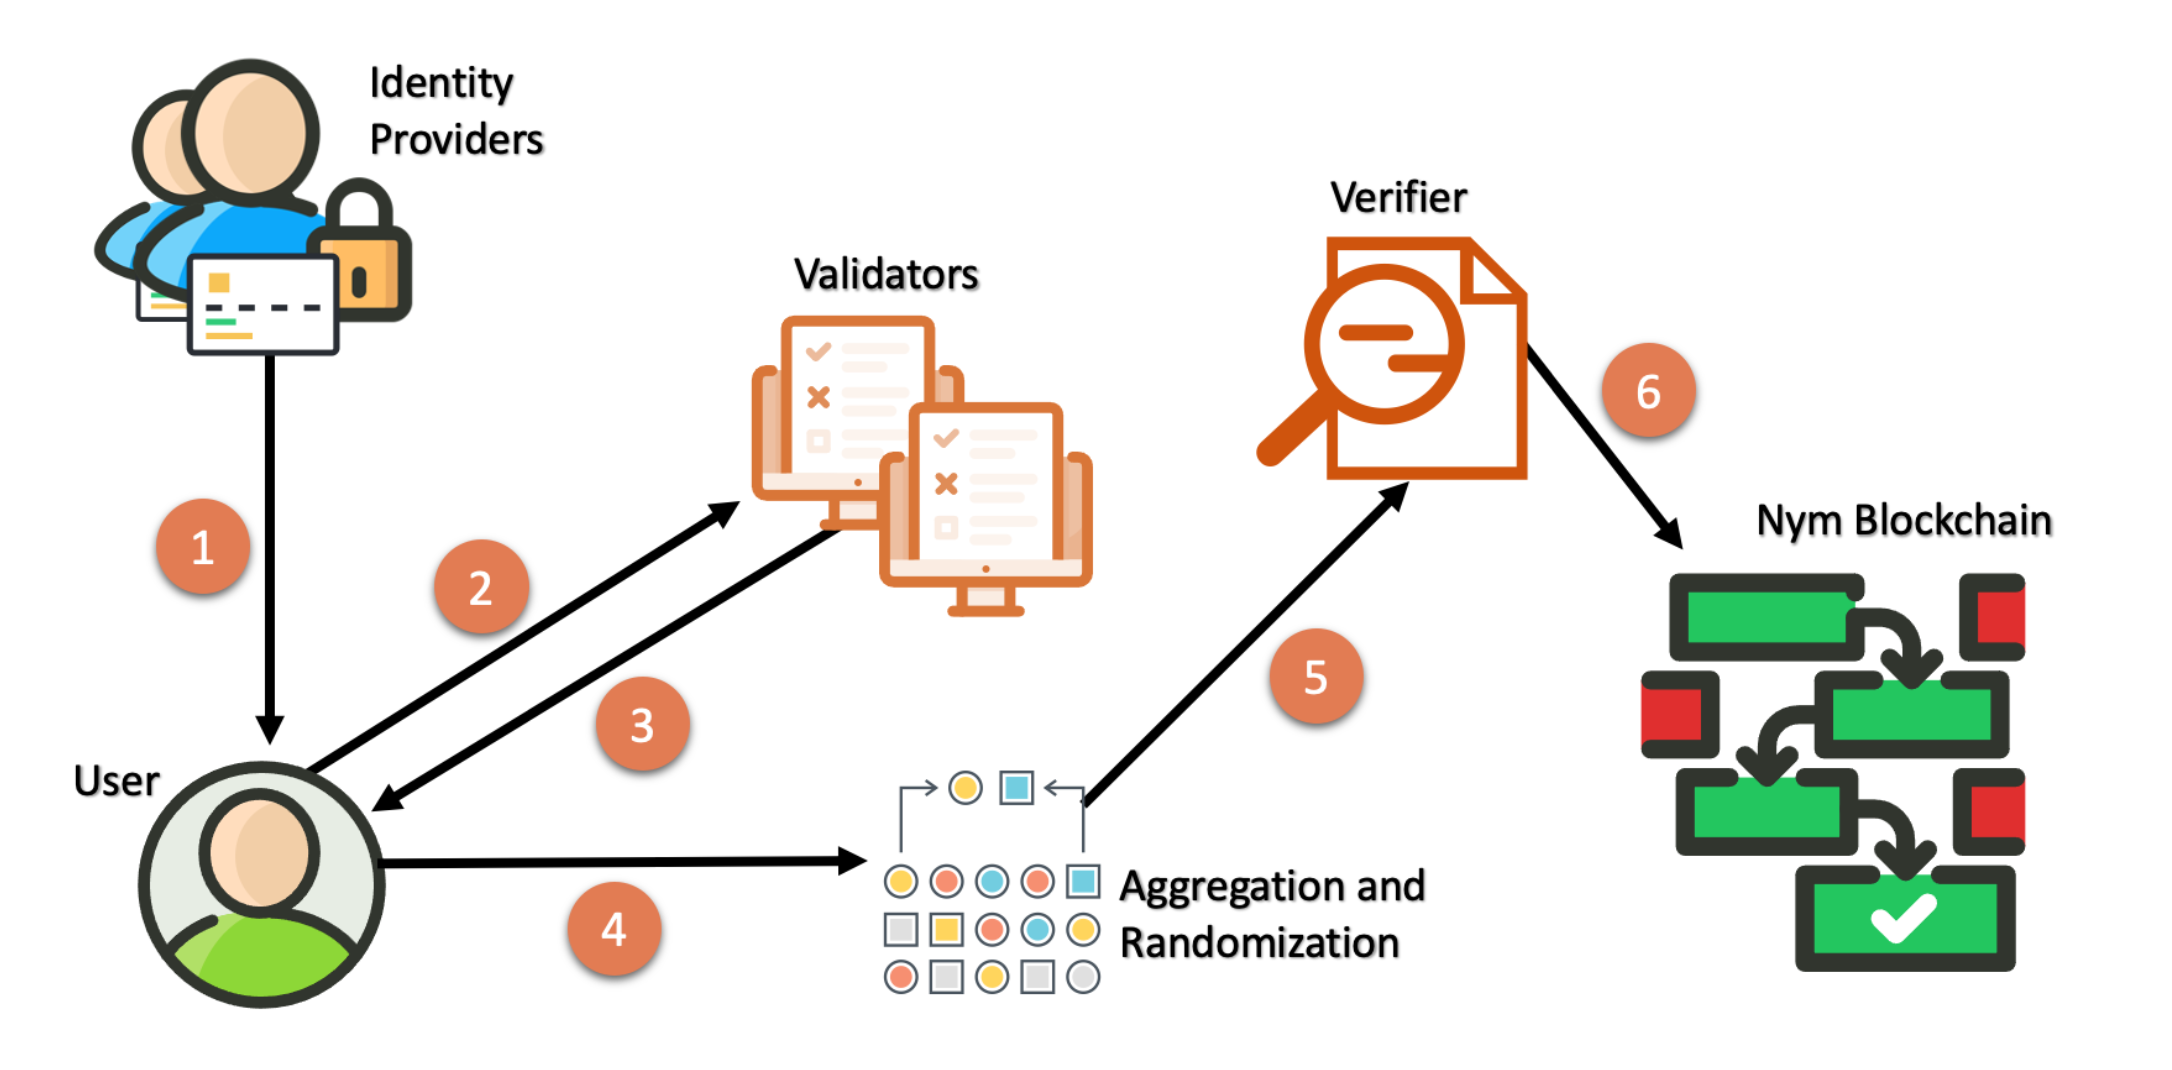
\includegraphics[width=1\textwidth]{image5.png} %1.png是图片文件的相对路径
\caption{获取和展示 Nym 凭据的步骤} %caption是图片的标题
\label{图 5} %此处的label相当于一个图片的专属标志,目的是方便上下文的引用
\end{figure}

	设置完成后,获取和使用 Nym 凭据的步骤如图 5 所示:
	
\begin{enumerate}[1. ]
\item 用户在凭证中对每个所需属性进行编码。如第 5.4 节所述,当用户需要提供涉及多个属性的复杂证明时,Nym 提供了将凭证绑定在一起的功能。根据用例,属性可能需要来自身份提供商的第三方认证,例如银行认证的 KYC/AML 状态、公共机构认证的出生日期、组织代表认证的组织成员身份,或卖家发放的折扣券。在其他情况下,属性可以由用户自我认证,例如,如果它们对用户偏好或密码知识进行编码。请注意,这第一步是可选的,因为一些验证者不需要存款证明以外的任何属性。
\item 为了获得证明用户在 nympool 中存款的有效带宽或服务凭证,用户首先生成代表存款金额的未签名凭证和凭证满足的零知识正确性证明。然后,用户向包含未签名凭证和零知识证明的验证器发送请求。
\item 如果验证器检查存款并验证证明时一切正确,他们会在凭证上使用部分签名 $\alpha_{i}$ 进行响应。为阈值 $t$ 数量的验证器获得部分签名。
\item 用户对这些 $t$ 数量的份额进行聚合产生了有效的凭证 $\alpha$。重要的是,用户重新随机化凭证以使其使用与涉及凭证的所有先前交互不可关联。
\item 用户向验证者展示凭证以证明他们对服务的“使用权”。凭证显示协议涉及零知识证明,证明用户持有满足服务访问要求的凭证,包括支付以及任何所需的身份验证属性。
\item 为防止双花攻击,在接受支付证明之前,验证者(比如网关和服务提供者)会在区块链中检查凭证尚未被标记为已使用。接受后,验证者在区块链中发布对凭证序列号的承诺,以防止它在另一个验证者处进行双花。
\end{enumerate}

	\subsection{凭证格式}

	Nym 将原始 Coconut 凭证 \cite{ref101} 修改为模块化格式,允许应用程序定义和发布自己的服务特定属性,并让它们与 Nym 发布的存款证明进行互操作。在 Coconut 中,验证密钥的大小取决于可以包含在凭证中的可能属性的总数,这消除了应用程序按需添加新属性的灵活性。相比之下,在 Nym 中,每个凭证只包含一个属性,并且可以通过相同的密钥材料将多个凭证链接在一起,每个凭证嵌入不同的属性。通过这种方式,Nym 凭证为证明属性的任意组合提供了更多的多功能性和效率,而无需强制验证器为每种新类型的属性设置更长的密钥。Nym 凭证包含具有以下五个字段的单个属性的信息,其中前两个以明文编码,后三个经过加密并且只能通过知识证明获得:\newline
	
\begin{itemize}
\item (公开的)\textbf{颁发epoch}[$epc$]:颁发凭证的时间间隔。它确定证书颁发者的公钥,这是验证证书所必需的。
\item (公开的)\textbf{属性类型}[$type$]:凭证类型的标识符;例如,带宽凭证、带有付款证明的服务凭证、出生日期等。
\item (私有的)\textbf{属性值}[$val$]:嵌入在凭证中的属性值;例如,带宽凭证中的“100 MB”数据,服务凭证的“50 NYM”存入代币,或出生日期的“1975-11-20”。
\item (私有的)\textbf{密钥}[$k$]:凭证的密钥,由用户随机生成,只有用户知道。需要此密钥来证明凭证所有权并将凭证捆绑在一起作为属于同一用户。
\item (私有的)\textbf{序列号}[$s$]:由用户生成且只有用户知道的随机数。此序列号用于防止涉及付款证明的凭据的双重花费。在旨在以不可链接的方式无限次显示的凭证中不需要该字段,例如年龄证明。
\end{itemize}

	\subsection{将多个凭证绑定在一起}

	Nym 是一个开放网络,服务提供商可以在其中定义自己的属性类型,并请求用户将它们包含在 Nym 凭证中以用于独立于 Nym 网络的授权目的。服务提供商要求的任意属性不是由 Nym 验证器发布或认证的。根据用例的不同,这些属性可能由第三方身份提供者或服务提供者自己签名,也可由用户自行认证。包含由不同发行者认证的属性的凭证的绑定是通过秘密凭证字段 $k$ 完成的。用户必须在他们想要绑定在一起的凭证中设置相同的密钥 $k$。然后他们可以证明(以零知识)他们拥有一组受相同 $k$ 约束的凭证。\newline

	为了说明这一点,请考虑服务提供商向参与促销活动的用户提供折扣的情况。该服务需要支付证明和参加活动的证明,但不需要知道用户的姓名或用户在活动中可能提供的任何其他个人信息。为此,用户的客户端在本地生成具有自定义属性类型“promotionXYZ”的自定义 Nym 凭证,该凭证具有随机生成的序列号 $s$。 凭证密钥 $k$ 被设置为与绑定用户不可转让凭证的秘密长期假名相匹配。根据促销组织者的标准,用户在参加活动时会获得他们的凭据。\newline

	在稍后的时间点,用户向 nympool 存入代币,并从验证器那里获得服务凭证,用于存入价值减去任何合适的费用。如果需要,用户执行拆分操作(第 5.5 节)以获得嵌入(确切)折扣促销率的服务凭证。重要的是,选择服务凭证的密钥 $k$ 以匹配自定义促销凭证中的密钥。在以折扣支付时,用户证明:(1)他们拥有有效的未使用的“promotionXYZ”凭证,(2)他们拥有用于确切折扣率的有效的未使用服务凭证,以及(3)两者凭证包含相同的密钥 $k$,因此属于同一用户,同时保持用户身份未知。\newline

	除了使凭证持有者能够证明他们满足涉及多个属性的授权条件外,凭证的密钥 $k$ 还可以作为一个隐藏的长期假名,防止凭证汇集和抑制凭证共享,同时保持凭证的匿名性所有者。\newline

	\subsection{拆分合并操作}

	如上所述,隐私是系统的整体属性,一个组件中的信息泄漏可能足以破坏不可链接性并使用户去匿名化。Nym 凭证依赖于在协议级别保证不可链接性的加密技术。然而,在编码支付证明的服务凭证的情况下,支付金额可能充当破坏隐私的侧信道。例如,如果每项服务收取不同的费用,则可以从用户在 nympool 中的存款金额推断出用户打算使用哪种服务。\newline

	Nym 凭证扩展了 Coconut 的功能,可以解决此问题:用户可以使用未使用凭证中编码的金额执行屏蔽拆分和合并操作。这些操作发生在加密域中,因此所涉及的金额受到保护。例如,这允许用户在一段时间内进行各种默认金额的存款,然后通过合并操作将它们以零知识聚合成一个用于支付昂贵服务的大凭证。用户还可以在 nympool 中存入默认的一次性代币,然后使用拆分来获得两个凭证:一个用于支付服务收取的确切金额,另一个包含他们保留以供以后使用的更改。通过这种方式,他们可以为多项服务的订阅付费,或者支付服务随时间向他们收取的经常性付款,直到他们消费完原始的一次性付款。最后,如果用户不再希望使用它来访问服务,也可以自己兑换未使用的凭证。\newline

	请注意,无法区分这两种情况,一是参与者正在恢复(部分)一个未使用的凭证,以证明自己未与他人一起花费存款的情况;二是参与者向他人提供服务而换取凭据的情况。这确保了所有获得凭证的用户都在其总存款的范围内混合到同一个匿名集合中。虽然应用程序的多样性必然需要定价金额的多样性,但存款应该具有取自一组固定金额(例如 10 的幂)的值,然后根据使用服务或支付后退零钱的需要执行拆分和合并操作。我们强调拆分和合并操作是在加密域中进行的,这意味着无法看到被拆分或合并的金额。给定一组存款和赎回凭证,一旦用户在存款和支付之间频繁进行拆分和合并操作,根据金额匹配它们就变得不可行。\newline

	拆分和合并功能由 Nym 验证器提供。希望合并两个(或更多)凭证的用户生成一个新的凭证 $\alpha_{3}$,其值为要合并的两个(或更多)凭证 $\alpha_{1}$ 和 $\alpha_{2}$ 的总和。用户向验证器发送 $\alpha_{3}$ 以及证明:
	
\begin{itemize}
\item $\alpha_{3}$中的 $val_{3}$ 值是这样的:$val_{3} = val_{1} + val_{2}$。
\item 序列号 $s_{1}$ 和 $s_{2}$(分别为 $\alpha_{1}$ 和 $\alpha_{2}$)未使用。
\end{itemize}

	如果一切都正确,验证器将 $s_{1}$ 和 $s_{2}$ 标记为已使用,并在新的合并凭证 $\alpha_{3}$ 上发出部分签名 $\alpha_{3,i}$。与前面的情况一样,用户聚合 $t$ 个部分签名以获得 $\alpha_{3}$,并随机化凭证以使后续交易不可链接。\newline

	类似地,用户可能希望将凭证 $\alpha_{1}$ 拆分为两个(或更多)较小的凭证 $\alpha_{2}$ 和 $\alpha_{3}$。这种情况的一个常见用例是用户拥有的凭证金额大于服务所需的金额,他希望将其分成两部分:一个用于立即付款,另一个用于保留零钱。为了拆分大凭证 $\alpha_{1}$,用户生成新凭证 $\alpha_{2}$ 和 $\alpha_{3}$,并将它们与证明一起发送给验证器:
	
\begin{itemize}
\item $val_{2}$ 和 $val_{3}$ 的值满足如下:$val_{2}\ge 0, val_{3}\ge 0, val_{1} = val_{2} + val_{3}$。
\item 序列号 $s_{1}$ 未使用。
\end{itemize}

	验证成功后,验证者将 $s_{1}$ 标记为已花费,并发出部分签名 $\alpha_{2,i}$ 和 $\alpha_{3,i}$。注意,用户可以任意组合拆分和合并操作,并提交一组未花费的输入凭证 {$\alpha_{in}$} 进行合并并拆分为一组输出凭证 {$\alpha_{out}$} ,这样(1) {$\alpha_{out}$} 中的所有值是非负的,并且(2) {$\alpha_{in}$}  中凭证的值的总和等于 {$\alpha_{out}$} 中的值的总和。\newline
	
	\subsection{凭证间隔}

	当 Nym 验证器集合更新时,用于签署凭据的阈值密钥也会更新,验证器用于检查验证器颁发的凭据的公共验证密钥也会更新。考虑到正常运行时间和服务质量会增加节点的声誉和选择验证器集的可能性,验证器节点预计将非常稳定。此外,所有验证器协议的阈值性质意味着即使多个验证器失败或同时受到攻击,验证器集也可以不受干扰地继续运行。鉴于此,验证器集更新的间隔可能比 mixnet epoch 更长。我们预计它们会在一周到一个月之间。\newline

	在更新验证器集时,凭证的公共验证密钥的版本再次构成潜在的侧信道。如果凭证根据其验证密钥是可区分的,该密钥与它们的颁发时间相关,那么每次更新验证器集时,都会对凭证匿名集进行分区。这种分区与在线活动时间相结合可能会使一些用户去匿名化。例如,考虑一个用户获得凭证,然后立即下线并长时间保持离线状态。到用户重新连接时,用户获得凭据时颁发的所有其他凭据都已使用。当她展示她的凭证时,可以通过看到她正在出示罕见的旧凭证来推断“匿名”用户的身份。\newline

	为了防止这种情况发生,Nym 要求凭据是最新的,以便验证者可以接受,验证者只接受验证密钥与当前验证者集相对应的凭据。拥有未使用的过期凭证的用户需要先使用验证器刷新它们,然后才能将它们与验证器一起使用。通过这种方式,所有颁发的凭据都聚合在一个大型匿名集中,该集合中随着时间的推移融合了所有用户,而不是将用户划分为在极端情况下可能导致用户识别的不相交的小型匿名集中。\newline

	为了刷新过时的凭证 $\alpha_{0}$,用户(或任何拥有凭证的参与者)有效地使用当前的一组验证器“销毁” $\alpha_{0}$,以换取等效的更新凭证 $\alpha_{1}$。为此,用户生成与旧凭证具有相同类型、值 $val$ 和密钥 $k$ 的新凭证。新凭证将发行周期 $epc$ 更新为当前周期并生成新的随机序列号 $s_{1}$。用户将新生成的凭证连同值 $val_{0} = val_{1}$ 和 $k_{0} = k_{1}$ 的证明一起发送给验证器。验证者检查序列号 $s_{0}$ 是否尚未被使用,并验证所提供的凭证和证明的正确性。如果 $\alpha_{0}$ 未花费且 $\alpha_{1}$ 正确,则验证器将 $s_{0}$ 标记为已花费并发布签名凭证份额 $\alpha_{1,i}$。用户再次聚合 $t$ 个份额来重建他们更新的凭证 $\alpha_{1}$。\newline

	验证者颁发的服务凭证对可赎回的代币存款进行编码。当用户向验证者展示服务凭证时,验证者会将凭证的序列号标记为已使用。 然后,验证者可以通过证明验证者签署了对其正在兑换的凭证序列号的承诺,从而与验证者一起兑换凭证。验证者还可以将一组凭证组合在一起,以隐藏每个凭证收到的单独金额,而不是证明所声称的总数的正确性。验证者检查所有证明的有效性,并将奖励从 nympool 转移到适当的接收者。这可能会以定期奖励间隔执行,以增加 nympool 存款和向服务提供商支付奖励之间的时间不可关联性。为简单起见,奖励间隔可能与凭证间隔相同,但如果有令人信服的理由,可以选择不同的间隔长度。\newline

	带宽凭证编码允许在凭证间隔期间通过 mixnet 发送数据包。显示的带宽凭证由网关收集并定期提交给验证器以在间隔结束时领取奖励。网关的奖励类似于混合节点,网关的奖励份额与其通过带宽凭证从其用户那里收集的带宽配额成正比,作为整个时间间隔内所有网关收集的总量的一小部分。请注意,用于交换带宽凭证的 nympool 存款以奖励的形式在所有 Nym 节点运营商(混合节点、网关和验证器)之间共享。也就是说,验证者不会以他们兑换服务提供商声明的服务凭证的方式直接向网关“退还”带宽凭证中编码的值。\newline

	\section{加密经济学}

	可扩展性和可持续性是 Nym 网络成功发展的必要特征。可扩展性是指支持具有大量用户群的广泛应用程序的能力。Nym 网络必须为服务提供可靠、高性能、高质量的隐私,并且即使在其某些组件出现拜占庭式故障时也能保持安全和运行。可靠地大规模提供隐私服务需要在带宽和计算方面的资源。可持续性确保 Nym 节点运营商可以支付他们在运行节点上的投资,并通过奖励从他们的劳动中获利。为了增长,网络需要增加更多容量以服务更多用户并隐蔽路由更多数据。Nym 利用密码经济学,在我们的案例中是密码学,以便服务提供商及其用户的需求为以可持续方式扩展网络所需的基础设施提供资金\cite{ref2}。\newline

	在 Tor 和比特币 \cite{ref40} 的发展之前,为混合节点提供准确的声誉分数的问题有助于决定将哪些节点包含在网络中。在混合网络的背景下,核心挑战是:我们如何证明混合节点通过正确遵循协议对路由做出贡献,并根据它们随着时间的推移提供隐私的程度来赋予它们声誉。声誉系统是针对 mixnet 进行理论化的,但没有一种有效且可扩展的方法来证明混合节点是否可靠,因此未能由打算发布可用软件的程序员实现\cite{ref44}。尽管已经在电子投票中使用的重新加密混合网络的可验证 shuffle 证明方面进行了工作,但这些方法仅适用于不能动态扩展的批处理混合网络,并且零知识证明的计算成本太高,无法为大量数据包生成 \cite{ref4}。为 mixnet 访问付费的概念早已被理论化\cite{ref47},Zero Knowledge Systems等初创公司也曾尝试构建商业混合服务\cite{ref48},但这些早期的尝试并没有成功,部分原因是缺乏隐私增强的数字支付系统(因为向中央公司支付匿名费用是有问题的)。以前激励 Tor 节点的尝试通常试图让用户以某种“逐跳”的方式奖励节点\cite{ref60},但这些类型的支付系统通常会损害隐私并导致攻击 \cite{ref64, ref91},因此 Tor 网络建立在没有任何支付基础设施来支撑节点运营商的基础之上。\newline

	Nym 网络以比特币的洞察为基础,将隐私作为一种共同利益,同时为提供这一关键基础设施的节点运营商提供回报和可持续性。受比特币交易费用的启发,需要在 Nym 存款才能获得带宽凭证并通过 Nym mixnet 进行隐私通信。为此,NYM的价值反映了对隐私的需求,因为可用的混合节点可以通过路由数据包来提供这种隐私服务。在需求方面,随着对隐私增强网络访问需求的增加,更多的 Nym 可以分配给 Nym 节点。更多的节点可以加入 Nym 网络以获得越来越多的奖励。这种机制设计的目标是让 Nym 网络能够动态扩展优质节点的供应,以满足隐私需求。\newline

	在供应方面,Nym 网络随着时间的推移标记节点的声誉。Nym 节点的声誉最终将与其未来可靠的网络容量供应预测相关联,它由节点自己的质押和其他利益相关者委托的代币的总和表示。任何想要自己运行节点的人都必须首先承诺一定数量的 Nym。这个承诺充当种子声誉(它是节点运营商投资加入和运营的“skin in game”,在极端情况下甚至可以被削减),它是一种防止女巫的措施,因为创建许多节点身份变得昂贵。除了节点承诺之外,所有 NYM持有者都可以委托其他人运行的候选节点,以此来提高候选节点的声誉,这反过来又决定了该节点在下一个时间间隔内被选为网络一部分的机会。当候选节点在网络中变得活跃并满足运营要求时,它会收到与支持该节点的代币委托人共享的奖励。使用第 6.4 节中描述的混合协议证明定期测量节点的服务质量,测量的节点性能对节点获得的奖励数量有直接影响。遭受频繁故障的节点无法获得奖励,这会抑制代币持有者委托给这些节点,降低他们的声誉并降低他们被选中的频率。最终,性能不佳的节点被排除在外,确保 Nym 网络的持续可靠性。\newline

	尽管 Nym 不是“权益证明”网络,但我们使用术语“权益”作为“声誉”的代理,因为 Nym 节点的奖励与其工作成比例,而不是其权益。Nym 运营商不是通过像比特币这样的哈希谜题来进行“工作证明”,而是执行 Nym 网络所需的资源密集型工作,以协作为服务提供隐私基础设施。混合节点因混合而不是挖矿而获得奖励。验证器通过签署数据块和凭证共享来工作。网关验证带宽凭证并路由进出混合网络的流量。股权用于表明节点声誉并确保激励节点运营商提供高质量的服务。更频繁地选择具有良好声誉的节点来执行工作并获得奖励。\newline

	Nym 网络从使用网络的费用中赚取收入,这包括购买带宽凭证以通过 mixnet 发送数据以及将存款转换为服务凭证的费用(请注意,服务凭证值可由凭证接收者赎回)。这些 nympool 存款用作在奖励间隔期间重新分配给活跃节点的奖励,保留一小部分作为储备以确保长期网络稳定性。与比特币挖矿奖励类似,节点运营商也从混合挖矿奖励中获得奖励。Mixmining 奖励来自一个池子,该池子在网络创始时使用大量 NYM进行初始化,这些代币随着时间的推移被释放,以通货紧缩的方式奖励节点运营商。预计混合挖矿资金最初将成为奖励的主要来源,随着时间的推移,随着混合挖矿奖励的下降以及更多应用程序和用户加入 Nym 网络,费用将取代混合挖矿成为节点运营商的主要收入来源。\newline

	在本节中,我们概述了用于自组织 Nym 网络的加密经济学。首先,我们在第 6.1 节中描述了 NYM的作用。接下来,在第 6.2 节中,我们解释了混合挖矿奖励如何激励 Nym 网络的引导,同时储备确保长期可持续性。然后我们从一个时代的角度来看 Nym 混合网络的生命周期。我们首先在第 6.3 节中展示节点如何加入 Nym 网络,然后在第 6.3 节中展示 NYM如何促进隐私增强带宽的拍卖,从而导致选择混合节点然后分配给网络。网络中的节点通过第 6.4 节中给出的 proof of minxing 协议来衡量其服务质量,并根据第 6.5 节获得奖励。在 epoch 结束时,Nym 网络会动态重新组织以匹配需求。\newline
	
	\subsection{Nym代币}

	所有参与者都需要 NYM 代币参与网络,该网络将在启动时全面运行。简而言之,NYM 奖励参与,帮助防止网络滥用,并在网络扩展以满足不断增长的需求时激励网络的可靠性和可用性。\newline

	利益相关者是持有 NYM 代币的所有参与者,这转化为用于选择哪些节点积极为网络做出贡献的声誉。根据他们的偏好和能力,一些 Nym 利益相关者自愿通过\textbf{质押} NYM代币作为他们的初始存款来运营混合节点,而其他人则审查节点统计数据和特征,以决定是否通过将他们的权益\textbf{委托}给某个节点来支持该节点,从而提高其声誉和被选中的机会。因此,“质押”NYM 是指这些操作:(1)设置节点并质押 NYM,或(2)审查节点特征并将 NYM 委托给现有节点,然后选择节点在网络中运行,其可能性与其总权益(质押和委托)成正比。\newline

	用户需要 NYM 代币才能通过 Nym 网络进行私密通信和访问服务。 然而,用户如何向服务和 Nym 网络本身付款取决于服务提供商。 例如,服务提供商可以为其所有用户批量赞助带宽,以便他们可以通过 Nym 网络轻松访问服务。 或者,用户可以在个人基础上支付类似于比特币交易费的额外“隐私费”。 虽然我们希望一些用户以比特币等加密货币支付访问 Nym 网络的费用,但 Nym 的用户可能会继续使用与其提供商的传统法定关系。 无论付款方式如何,从存款中收取的费用都会转换为 NYM,以衡量对隐私的需求并通过奖励维持 Nym 网络。 费用在奖励间隔期间在 nympool 中收取,然后在间隔结束时以奖励的形式分配,如第 6.5 节所述。\newline

	NYM代币是 Nym 网络运行所必需的加密资产。代币代表 Nym 网络提供的经济价值,并为提供 Nym 网络生成的隐私的节点提供奖励。我们不认为 NYM 被用作 Nym 网络之外的加密货币。总的来说,它的主要用途是平衡 Nym 网络对隐私的供求。Nym 用户可以继续使用法币支付服务费用,一些高级用户更愿意使用已经隐私的加密货币来支付服务费用。我们不希望限制服务如何接收付款以及它们可能具有的任何付款条件,因为它有利于所有人的隐私,以最大限度地增加 Nym 网络上的服务和用户数量。同样,Nym 服务凭证可用作比特币、法定货币或服务接受的任何其他加密货币的“付款证明”,它们可以包含服务提供商所需的任何其他附加信息。Nym 节点也可能希望使用他们的 NYM代币来获得维持和增加他们在网络中的作用所必需的资源,因此 Nym 运营商可能选择以比特币或另一种(可能是隐私的)加密货币接收付款,而不是将他们的奖励保留在 NYM代币。NYM的主要功能现在或将来都不会用作获取商品或服务的支付手段,以及货币或价值转移的手段。NYM 代币可以是支付交易费用的一种支付方式,但仅限于 Nym 网络内。通过使用比特币作为支付手段的加密货币,Nym 可以在使用 Liquid \cite{ref3} 等高级功能的同时支持比特币。这种设计还允许 Nym mixnet 与任何底层区块链无关,并支持最大数量的服务,以最大限度地保护所有用户的隐私。\newline

	\subsection{混合挖矿奖励和储备}

	定期分配给节点运营商的奖励是支付给网络的 nympool 中的混合挖矿奖励和费用的总和。混合挖矿释放计划旨在使节点运营商在网络启动时超越其盈亏平衡点,并在网络的整个生命周期内保持盈利。我们预计混合挖矿池将成为网络生命周期最初几年的主要奖励来源,随着网络以与比特币类似的方式吸引更多使用,费用收入将接管。此奖励计划的精确加密经济学将在单独的文档中详细说明。\newline

	如果混合挖矿池完全耗尽,Nym 网络将没有资源可以从暂时的需求下降(以及相应的费用收入中断)中恢复过来。为防止这种情况发生,一小部分获得的费用将退回到长期储备中。然后,该储备可用于在需求突然下降的情况下稳定节点回报。该储备预计由利益相关者管理。请注意,混合挖矿池、储备和代币发布时间表的详细信息和精确参数在单独的加密经济文档中。\newline

	\subsection{加入Nym mixnet:定价带宽和节点选择}

	在每个时间段内选择在 Nym 网络中运行的节点依赖于市场机制。作为初步事项,需要对预期的所需容量进行估计,以决定应该选择组成混合网络的混合节点的数量。在 Nym 中,这是根据网关声称的最近使用带宽凭证的历史来预测的,网关提供了每个 epoch 通过网络发送的数据包数量的上限。\newline

	希望运行混合节点的运营商提交一份声明,说明他们的每包价格 $(PP)$ 函数以及要应用于节点收入的利润率 $(PM)$。另一方面,验证器只是简单地说明维护其验证器服务器以及签署凭据和数据块的固定成本。如第 5.6 节所述,网关根据从用户那里收集的带宽凭证按比例获得奖励。对于混合节点,$PP$ 函数将路由数据包的数量映射到节点运营商每个数据包花费的 Nym 数量。它还隐含地定义了节点的容量 $c$ 。$PP(0)$ 表示没有路由任何数据包的裸操作成本,而当 $x$ 超过节点的容量 $c$ 时, $PP(x) = ∞$。\newline

	Nym 网络可能会规定每个节点必须提供的最低容量,并规定每个节点可接受的最大容量。如果一个节点声明 $PP$ 高于最小容量,则可以认为它已注册到 Nym 网络并可能被选择在网络中运行。如果(如预期的那样)注册的节点多于需要的数量,则网络选择节点的概率与其质押的(质押加委托的)NYM数量成正比,因为这是来自节点声誉市场的“信号”。\newline

	给定混合节点声明,我们可以推断出一个中值节点函数 $PP_{med}(w) = median\left \{PP(w)  \right \} $,其中中值在给定的每 epoch 流量负载 $w$ 的所有提交的声明中运行。现在假设我们希望按照带宽凭证定价的要求,预先根据带宽对工作单元进行定价。如果有一个带有定价声明 $PP()$ 的单个节点来处理整个工作,那么可以使用的特定方案如下。假设实际需求服从概率分布 $\mathcal{D}$。我们用 $W$ 表示服从分布 $\mathcal{D}$ 的工作的随机变量。第 $x$ 个工作单位的价格定义如下:

\begin{equation}\nonumber
PP(x)-P P(x-1)+P P(0) \cdot \frac{1}{\mathbb{E}[\mathrm{W}]}
\end{equation}

	在上述定价方案下,节点的预期收益为$\mathbb{E}[PP(\mathrm{W})]$,其中 $W$ 是根据 $\mathcal{D}$ 分配的工作的随机变量。

	对上述事实的简单证明有助于阐明带宽凭证定价设置合理的原因。将所有销售的工作单位相加,收入将等于:
	
\begin{equation}\nonumber
\mathrm{W} \cdot PP(0) / \mathbb{E}[\mathcal{D}]+\sum_{x=1}^{\mathrm{W}}(PP(x)-PP(x-1))=\mathrm{W} \cdot PP(0) / \mathbb{E}[\mathrm{W}]+PP(\mathrm{W})-PP(0)
\end{equation}

	通过期望的线性,我们得出该陈述的正确性,并且作为推论,只要 $\mathcal{D}$ 的方差很小,每单位定价方案就会收支平衡。我们注意到这是一个简单的线性方案,适应更复杂的模型\cite{ref5, ref67}也是可能的。\newline

	由于上述方程描述了单个假设混合节点的定价方案,对于整个 Nym mixnet,我们使用下面的修改公式,该公式考虑到 mixnet 具有 L 层(因此工作量乘以 L)而负载由每层内的节点容量平衡。使用中位数 $PP_{med}()$ 数据包价格公式:

\begin{equation}\nonumber
L \cdot\left(PP_{\operatorname{med}}(\lceil x / W\rceil)-PP_{\operatorname{med}}(\lceil x / W\rceil-1)+PP_{\operatorname{med}}(0) \cdot \frac{1}{\mathbb{E}[\mathrm{W}]}\right)
\end{equation}

	基于以上所有,我们观察到混合节点之间的微小变化、合理集中的需求函数和平滑的 $PP(·)$ 定价函数导致带宽凭证产生的总收入抵消了运营成本的情况。混合网络作为一个整体,在需求变化较大的情况下,$\mathcal{D}$ 有较大的方差,会导致节点收入的较大方差,混合挖矿奖励可以帮助维持定价的稳定性\cite{ref59}。\newline

	在每个 epoch,$k$ 个节点被注册并可用作混合节点,其中 $k$ 是一个动态调整的参数。下面,我们将描述填充 mixnet 的机制; 选择和奖励验证者的过程是类似的。一些节点被选为在 mixnet 中运行,而其他节点则在形成“储备”的 epoch 中处于空闲状态。如果 $r$ 表示保留节点的数量,则混合网络中每层平均有 $(k − r)/L$ 个活动节点。节点的选择是概率性的,使用无替换的随机抽样,并且节点选择权重与其质押的 NYM成正比。 一旦选择了下一个 epoch 的节点集,节点就会随机分配到 mixnet 层,以防止对手战略性地定位受损节点。\newline

	“质押”在节点上的 NYM是衡量节点声誉的指标。因此,通过权益权衡选择将哪些混合节点包含在网络拓扑中,会导致混合网络由具有提供高质量服务的声誉的节点组成。如果混合节点在 NYM中拥有大量委托权益,这表明社区支持该节点的声誉,因为该节点始终可靠地在线并保持良好的性能而定期为其委托者提供奖励 。此外,这种节点选择过程还优化了用户的成本,有利于可靠且经济高效地选择混合节点。声明 $PP$ 函数过于昂贵的混合节点将向委托分配较低的奖励,因为 $PP$ 越低,节点的委托者可获得的奖励越高。\newline

	为了吸引委托者,新的混合节点必须提供有吸引力的参数:要么提供更具竞争力的 $PP(·)$ 和 $PM$,从而为委托者留下更多的奖励份额,要么引入其他有吸引力的外部性,例如将一些收益捐给诸如人权活动家,使其可以“免费进入”Nym,这将引起一些代表的共鸣。回想一下,表现不佳的节点收到的奖励减少或没有奖励,导致委托者不再支持它们。这可能是自愿发生的,因为奖励下降,或者是强制发生的,比如混合节点的注册因性能不佳而被撤销。这为新的混合节点创造了吸引失败节点的现有委托者的机会。目标是,随着时间的推移,Nym 网络将收敛于为用户提供隐私的最佳价格。\newline

	\subsection{Proof of mixing}

	Nym 的生存能力的关键在于节点提供始终如一的高质量服务 (QoS),例如混合节点正确可靠地处理、路由和传递消息。性能因子 $PF$ 表示混合节点正确路由消息的比例。Nym 将奖励分配给满足 QoS 标准($PF$ 接近 1)的节点,这增加了对每个节点进行可靠测量以估计 $PF$ 的需求。\newline

	以去中心化的方式为混合节点获得准确可靠的 $PF$ 测量是一项挑战,特别是当我们考虑到对抗性参与者的子集可能串通进行主动和战略性地尝试偏置测量时。部分挑战来自于 mixnet 内的通信仅对参与流量交换的两个实体(和网络对手)可见,而对其他实体不可见。因此,对于混合节点是否可靠地路由它们接收的流量,没有集体可见性,这意味着它们可以丢弃或不充分延迟数据包。此外,在 Nym 中,节点性能的测量不能依赖受信任的测量服务器(Tor采用的解决方案),因为这会引入一个中心化组件(和单点故障)控制一个非常重要的网络功能,决定谁获得奖励和奖励的多少。\newline

	混合节点运营商在通过 $PP$ 函数加入 Nym 网络时自行声明其容量。另一方面,它们的 $PF$ 是以去中心化的方式连续测量的。夸大其容量以试图获得更大份额奖励的节点在以其声明的容量使用时无法维持高 $PF$ 。并非增加收入,夸大容量反而会导致节点错失奖励并失去声誉。\newline

	在电子投票文献中,存在混合节点设计,可以产生可验证的混合证明\cite{ref1, ref4, ref50}。然而,这种可验证性需要付出巨大的代价。这些混合是缓慢的、基于批处理的,需要昂贵的最终阈值解密,并且需要混合节点不直接通信,而是通过可公开验证的广播通道(例如区块链)发布所有输入和输出消息,以及对于网络中的每个混合节点和每批消息的输入和输出消息批次之间正确排列的零知识证明。虽然这些限制和成本对于投票用例来说是可以容忍的,但它们对于我们的目的、部署上下文和应用程序要求来说是不切实际的。因此,为了准确估计混合节点丢弃数据包的速率(无论这是恶意的还是仅仅由于缺乏资源),我们采用一种普遍可验证但去中心化的方式对其性能进行采样。这是通过使用特殊的 Sphinx 编码的测量消息来完成的,这些消息在通过 mixnet 传输时与所有其他消息无法区分,并且仅在 epoch 结束后作为测量消息显示。\newline

	\textbf{1. 测量消息的生成。}测量消息由混合节点和终端用户生成,遵循与虚拟环路消息相同的循环路由。终端用户需要生成一些测量消息的原因是为了端到端地测量与其他类型的流量(例如应用消息、确认和覆盖流量的循环)完全无法区分的流量的 QoS。\newline

	为了确保参与者不能(可能是恶意地)偏离测量消息的时间和路由,这些消息是使用可验证随机函数(VRF)\cite{ref80} 和采样器伪随机生成的。我们认为测量协议中的所有参与者都有一个公钥对 $(pk, sk)$,可以验证地与其在 Nym 网络中的角色相关联。Nym 节点和可公开访问的服务提供商的公钥通过区块链分发,作为网络公钥发现的一部分。终端用户需要拥有一个有效的带宽凭证来生成测量消息,用于生成测量消息的 VRF 密钥与凭证中包含的密钥材料绑定。\newline

	在每个 epoch 之前,验证者联合发布一个随机信标 $x$。每个参与者 $i$ 计算 VRF 输出 $y_{i}$ 和相关证明 $\pi_{i}$,它们对应于输入 $x$ 与他们的私钥 $sk_{i}$ 的结合,即 $y_{i}, \pi_{i} \leftarrow V R F\left(x, s k_{i}\right)$。请注意,具体实现可以使用确定性地从 $x$ ,而不是 $x$ 本身导出的输入;例如,$x$ 由标签连接,以获得与用于其他目的的 VRF 输出不同的 VRF 输出;例如,随机化混合网络拓扑。参与者然后用他们的 $y_{i}$ 和关于网络的公共信息(混合节点描述符和网络参数)为采样器做种子。该采样器输出伪随机值以创建有效的 sphinx 数据包:随机循环组元素、通过 mixnet 层的路径选择、每跳的指数延迟以及应发送消息的时间窗口。\newline

	测量消息中的所有参数都是从采样器中伪随机导出的,这一事实使得这些消息在给定 $y_{i}$ 下,在发送时间、通过网络的完整路径、每跳产生的延迟以及用于导出每跳共享密钥的随机性方面可重现,所有这些都适用于转发数据包和嵌入其中的任何 SURB。这实现了公共可验证性,确保参与者不能恶意制作测量消息的有效标头。请注意,网关的选择不是采样器输出的一部分。这是因为参与者必须可以自由地通过他们用于其他流量的网关发送测量消息,这不是公共信息,因此采样器不知道。发送方和网关之间的通信使用对称会话密钥加密,但网关实际上不执行任何 Sphinx 处理操作; 相反,他们只是将接收到的 Sphinx 数据包转发到 mixnet。\newline

	\textbf{2. 路由测量消息。}在消息有效的 epoch 开始之前,所有参与者在本地提前生成他们的测量消息。一旦 epoch 开始,参与者就会在采样器确定的时间窗口内发送他们的测量消息。这些消息是 Sphinx 加密的,与在 mixnet 中路由的任何其他消息无法区分,因此它们通常通过网络路由。\newline

	作为 Sphinx 重放保护机制的一部分,混合节点会跟踪它们所看到的消息,这些消息由每跳回复标签标识。这样,如果一条消息被重放,就会有一条记录表明该消息在那个 epoch 中已经被看到,这使得识别和丢弃重复项成为可能。Nym $PF$ 采样方法搭载了这种重放保护机制。除了保留所见标签的列表之外,混合节点还将这些标签(连同标识何时接收和发送消息的时间戳)添加到本地 Merkle 树中。在 epoch 结束时,他们通过将其广播给验证器来提交该 Merkle 树的根,验证器将其发布在区块链中。请注意,未能广播 Merkle 根将导致混合节点被视为该 epoch 的 $PF = 0$,因此不会收到任何奖励。\newline

	\textbf{3. 打开测量消息。}一旦所有混合节点的 Merkle 根发布,所有测量参与者向验证器提交他们的 VRF 伪随机种子 $y_{i}$ 和相应的正确性证明 $\pi_{i}$。验证器在区块链中发布这些信息,通过将每个参与者的 $y_{i}$ 与公共网络信息一起提供给采样器,使每个人都可以验证种子的正确性并重新构建在 epoch 中生成的测量消息。然后混合节点检查哪些测量消息在路由中包含了它们自己的地址。对于那些这样做的人,他们会检查他们是否记录了该消息标签。对于正确的情况,他们打开 Merkle 树中的相应叶子,以证明他们已经提交了该消息标签以及时间戳,从而向每个人证明在消息被揭示之前已经处理了该消息,并且这是一条测量消息。请注意,混合节点有强烈的动机在其 Merkle 树中打开测量消息,因为不这样做会降低它们的性能指标,从而降低它们的奖励。\newline

	\textbf{4. 服务质量评估。}基于种子 $y_{i}$ 和 Merkle 树的打开,所有参与者都可以验证混合节点报告发送和接收了哪些消息,报告了哪些消息在哪些链接中丢失,以及哪些消息在某些跃点上延迟不足。请注意,测量方法会生成丢失消息的两个网络实体之间的链接,而不是暴露丢失消息的实体。这是因为无法区分以下两种情况,一是节点将标签添加到其本地 Merkle 树并随后丢弃数据包(因此自身对丢失负责);二是节点将标签添加到其本地 Merkle 树并成功发送数据包,然后在记录标签之前被后继者丢失(在这种情况下,后继者对丢失负责)。为了统计确定哪些节点对消息丢失负责,采样器确保测量消息测试一个 epoch 内的所有路由组合,此外还跨 epoch 重新组织 mixnet 以使用不同的拓扑配置进行测量。\newline

	\subsection{Epoch 奖励分配机制}

	在每个奖励间隔结束时,奖励数量 $R$ 可用于分配给节点,节点随后与通过委托权益支持他们的利益相关者分享一部分,从而提高他们的声誉。奖励 $R$ 包括来自 nympool 存款的费用(有效需求)以及混合挖矿奖励(通货膨胀)。奖励分配机制的目标是补偿执行混合用户流量工作的节点和支持良好节点运营商的委托者。为简洁起见,在本节中,我们将仅描述混合节点的奖励计算机制,类似的机制也适用于验证器。\newline

	该机制的目标是激励收敛到具有以下属性的均衡:
	
\begin{itemize}
\item 有 $k$ 个连续运行的节点(其中 $k$ 是一个参数,它取决于用户对流量的需求、mixnet 的拓扑以及为快速增长的需求而保持储备所需的节点),每个节点都拥有相当于总权益 $1/k$ 的委托权益。
\item 所有委托者每单位权益获得相同的奖励。
\item 委托给每个节点的权益对应于社区对其运营商的信任,并且这对节点的特定容量或成本效益不敏感(如果节点具有足够的竞争力,可以被选入 mixnet)。
\item 节点如果长时间停机或以其他方式偏离正确的混合操作,会失去其委托的权益。
\item 更具竞争力的节点(例如,成本较低的节点)能够将其竞争力转化为通过要求更高的利润率来获得更高的利润。
\item 公开或秘密注册多个节点的运营商(相当于女巫攻击)将受到惩罚,因为他们的节点奖励相对于他们仅注册一个节点所获得的奖励有所减少。这是因为将权益分成多个质押会导致整体回报较低。
\end{itemize}

	为实现上述目的,该机制以某种方式约束每个节点的奖励,并将它们与节点运营商质押的权益和委托给节点的权益相关联。该约束创建了一个"软上限",即向节点委派多少权益是合理的,将利益相关者推向目标混合节点数背后的公平组织,并防止仅将权益集中在几个节点上或提出太多碎片化的弱节点。更详细的说,机制如下:
	
\begin{enumerate}[1. ]
\item 该机制使用两个参数 $\alpha > 0$、$k \in \mathbb{N}$。有 $k$ 个节点需要补偿。它是\cite{ref10}的机制的一个实例化,通过设置每个 epoch 中节点执行不同数量的工作。参数 $k$ 设置了利益相关者被激励创建的节点数,因为当混合网络收敛到 $k$ 个节点时,奖励会最大化。参数 $k$ 以及处于活动和保留状态的节点数的确切选择,取决于预期的容量需求和 mixnet 层数。例如,如果我们想要 10 Mbs 的吞吐量,每个节点在具有三层的混合网中至少提供 1 Mbs,我们可以选择 $k = 100$,它可容纳 30 个操作节点,$r = 70$ 个备用空闲节点。参数 $\alpha$ 与系统的女巫弹性有关。
\item 第 $i$ 个节点发送的数据包数量用 $w_{i}$ 表示。请注意,如果 $w_{i} = 0$,这意味着该节点被选择为该 epoch 的保留节点。基于 $w_{i}$,确定一个分数 $w_{i}$,它指定第 $i$ 个节点承担的总工作量的分数(例如,如果没有人空闲并且每个人都发送相同数量的数据包,我们有 $w_{i} = 1/k$ )。记住,$\sum_{i=1}^{k} \omega_{i}=1$ 。
\item 使用第 6.2 节中给出的“proof of mixing”协议为每个节点计算性能因子 $(PF )$,该协议会按比例影响其奖励。对于新的混合节点,可以给出一个宽限期,其中 $PF = 1$。在每个 epoch 之后,根据混合证明确定的节点性能调整 $PF$ 的值。如果一个节点在多个 epoch 中表现不佳(这是一个系统参数),Nym 网络将采取额外的措施,从符合条件的节点集中删除拜占庭节点并暂时撤销其注册,请求节点修复所有技术问题。如果节点继续无法运行,可以通过冻结或削减其承诺来禁止节点运营商重新注册。
\item 分配给第 $i$ 个节点及其委托者的奖励金额等于:
\begin{equation}\nonumber
   R_{i}=P F_{i} \cdot R \cdot\left(\sigma_{i}^{\prime} \cdot\left(\omega_{i} \cdot k\right)+\alpha \cdot \lambda_{i}^{\prime}\right) /(1+\alpha),
\end{equation}
   其中 $\sigma_{i}$ 是委托给第 $i$ 个节点的总权益,$\lambda_{i}$ 是运营商向其节点质押的权益,$\sigma_{i}^{\prime}=\min \left\{\sigma_{i}, 1 / k\right\}$ 和 $\lambda_{i}^{\prime}=\min \left\{\lambda_{i}, 1 / k\right\}$ 。我们观察到以下预算平衡属性:
\begin{equation}\nonumber
   \sum_{i=1}^{k} R_{i} \leq R.
\end{equation}
   同时,$\sum_{i=1}^{k} \omega_{i}=1, \sum_{i=1}^{k} \lambda_{i} \leq 1 \text { and }\left(\sigma_{i}^{\prime} \cdot k\right) \leq 1 \text { for } i=1, \ldots, k$ 。请注意,以上确保没有激励将超过 $1/k$ 的总权益委托给一个节点,并且激励利益相关者创建 $k$ 个节点。
\item 鉴于上述情况,第 $i$ 个运营商被记入以下数额:
\begin{equation}\nonumber
   \left[\min \left\{P P\left(w_{i}\right), R_{i}\right\}+\left(P M_{i}+\left(1-P M_{i}\right) \cdot\left(\lambda_{i} / \sigma_{i}\right)\right) \cdot\left(R_{i}-P P\left(w_{i}\right)\right)\right]^{+},
\end{equation}
   其中,$[\cdot]^{+}=\max \{0, \cdot\}$ ,$PM_{i}$ 是第 $i$ 个运营商的申报利润率,而拥有委托权益 $s$ 的委托人,则收到
\begin{equation}\nonumber
   \left[\left(1-P M_{i}\right) \cdot\left(s / \sigma_{i}\right) \cdot\left(R_{i}-P P\left(w_{i}\right)\right)\right]^{+},
\end{equation}
\item 上述分配过程可能会产生剩余资金。当某些奖励由于节点低于“饱和”(即,它们的权益量小于 $1/k$)或它们的性能低于标准值而无人认领时,就会发生这种情况。这些剩余的资金将返回到储备中,将来可以在那里领取,以在需求暂时下降的情况下稳定奖励并留住节点运营商。
\end{enumerate}

	参数 $\alpha$ 激励质押,可用于减轻女巫攻击。其他女巫攻击缓解措施隐含在激励机制中,例如利益相关者为做出权益授权决定而进行的筛选。参数 $\alpha$ 提供的机制不是利益相关者筛选的替代,而是一种补充机制。请注意, $\alpha$ 的值越高,机制就越倾向于高质押的运营商,而 $\alpha$ 的值越低,机制就越倾向于最高效的运营商。观察到在 $\sum_{i} \lambda_{i}<1$ 的典型情况下,一部分奖励将保持无人认领并退回储备。\newline

	$k$ 的值以及空闲节点的百分比将定期(例如每月)调整,调整基于混合网络容量的预测需求。请注意,调整 $k$ 需要委托者采取行动以收敛到新的平衡,因此利益相关者应积极参与判断节点的声誉以做出授权决定。虽然利益相关者的不作为无害,但会导致较少的奖励。\newline

	\section{结论}

	互联网曾被誉为人类与技术共同进化的一大进步\cite{ref73}。它旨在提供对信息的普遍访问,建立全球对话以及以以前无法想象的规模进行集体自决的可能性。然后,相反的是,它正在成为控制社会的基础设施。元数据分析是这个过程中的关键,元数据分析是这个过程中的关键,因为它在预测并从而控制人类行为方面比内容分析更具预测性。\cite{ref85}。\newline

	但互联网并不注定是一台监控机器,还是有别的出路的。关键在于几乎被遗忘的工作。在互联网诞生之际,一小群先驱者——赛博朋克——意识到互联网可以转变为一个以前从未想象过的规模的监控网络,并着手提出解决方案。\newline

	\emph{Nym}这个词来自希腊语,意思是“名字”。在 1990 年代,它首先被用作早期赛博朋克 re-mailers(如 Mixmaster)中的一个艺术术语\cite{ref23}。正如 \emph{True Nyms and Cryptoaarchy} 所概述的那样,“数字假名,即创建无法被他人伪造但与其所有者的‘真实姓名’无关的持久网络角色”,这对于“确保言论自由、允许发表有争议的意见并提供无法阻止的经济交易”来说至关重要\cite{ref78}。几十年来,隐私增强型互联网的关键组成部分——数字现金、匿名凭证和混合网络——从未完全组装成一个可用的平台。尽管像 Zero Knowledge Systems 这样的初创公司在 1990 年代后期最初的“互联网”繁荣期间部署了商业混合网络,但由于缺乏像比特币这样的数字现金,导致在 2000 年代初期未能得到广泛采用。与此同时,Tor 所展示的非营利性资助模式已经产生了不需要解决声誉、激励和经济可持续性问题的众包或政府补贴的隐私增强技术。\newline

	在应对这些挑战时,Nym 可以为安全和隐私互联网奠定基础,使用户能够在不受监控和跟踪的情况下访问服务。虽然 Tor 和 p2p 系统仅旨在抵御弱威胁模型,但 mixnets 可以提供抵抗对整个网络上的所有活动具有上帝视角的对手。尽管这些对手曾经看起来可能过于偏执,但斯诺登的揭露表明美国国家安全局拥有这些能力。随着大数据和人工智能的兴起,越来越多的参与者可以部署这些能力,从小型民族国家到商业企业和能力超强的个人。\newline

	Mixnets 是目前唯一已知的大规模流量分析工作解决方案。在 Nym 之前,mixnets 的缺点之一是需要昂贵的计算才能使网络流量隐私。通过 NYM对声誉进行代币化是一项核心突破,因为它使提供隐私所需的计算变得有利可图,并且可以任意扩展以满足需求。代币化奖励确保 Nym 网络中的每个组件都有提供隐私的动机。赚取和使用 Nym 的循环使用户、服务提供商和 Nym 网络本身之间建立了互惠互利的关系。第二个核心突破是在混合协议的证明中使用统计采样,这使 Nym 能够在混合中实现高度的可靠性和服务质量,而无需缓慢且昂贵的加密技术。Nym 通过轻量级统计采样进行路由验证,而不是强制执行哈希谜题的计算成本高昂的任务,从而避免了过度的环境后果。Nym 产生的能源成本是由于以混合包的形式提供有用的工作。\newline

	开发人员可以在 Nym 之上构建许多重要的应用程序。 其中一些应用程序可以省钱,其他应用程序可以挽救生命。例如:
	
\begin{itemize}
\item \emph{加密货币钱包:}虽然有一些启用 Tor 的加密货币钱包,但仍需要隐私增强型钱包,以在网络级别启用私人交易和隐私,以保护用户身份免受第三方影响。
\item \emph{DeFi:}去中心化金融需要交易不可区分,包括网络级别的发送方匿名,以防止抢先交易并启用黑池,就像成熟的机构市场一样。
\item \emph{支付通道:}由于其网络结构,链下支付通道容易受到许多攻击,混合网络可以改善这些攻击\cite{ref64}。
\item \emph{安全消息传递:}当前的安全消息传递应用程序使用复杂的端到端加密,但元数据公开并且不抵制对其服务器的流量分析。
\item \emph{文件共享:}在某些情况下,以保持发送者和接收者匿名的方式共享敏感的大文件很重要。例如,在记者和举报人之间的交流中。
\item \emph{身份管理:}个人数据,如医疗记录,将受益于匿名凭证和网络级隐私的使用,以防止身份盗用和算法歧视。
\item \emph{多媒体流:}音频和视频会议越来越多地用于高度敏感的通信;因为它们可以容忍数据包丢失和无序到达,所以这些通信协议适用于混合网络\cite{ref27}。
\end{itemize}

	我们的目标是让 Nym mixnet 为大部分互联网提供隐私的未来,其中基于消息的路由在从即时消息到加密货币交易的领域变得越来越重要。这是合理的,因为与大多数区块链设计不同,Nym 是横向扩展的。就像网站可以通过添加额外的 Web 服务器来增加容量一样,Nym 可以通过添加新的混合节点来处理更多的流量。随着更多用户加入网络,Nym 可以加快速度并变得更加高效,因为更多用户在整个 mixnet 上的参与使得通过更小的混合延迟和更低的覆盖流量来实现相同程度的隐私成为可能。其他技术,例如 Tor 及其基于电路的路由,最终可能更适合 Web 浏览等用例,尽管它们的威胁模型较弱。\newline

	Nym 旨在以尊重其基本工程价值的方式升级互联网,实现组件的完全去中心化,同时激励开发人员利用 Nym 的技术构建下一代隐私增强应用程序。这听起来可能雄心勃勃,但之前已经有人做过,作为一个运行在现有互联网之上的覆盖网络,Nym 可以像 TLS 在互联网上传播加密数据一样的方式添加用户和应用程序,从一个应用程序开始,随着越来越多的应用程序需要改进隐私。我们设想 Nym 的广泛采用将从涉及对隐私的高需求的应用程序开始,例如加密货币,然后发展为更通用的应用程序,例如安全消息传递和去中心化 VPN。\newline

	尽管它比任何竞争对手都更详细,但这里提出的设计并不完整,还有很多工作要做。随着我们继续构建 Nym 网络,我们将对每个组件进行全面分析,并提供安全论据和证明,包括通过模拟对性能和匿名权衡进行实证分析。赛博朋克们编写代码,因为代码对现实世界的影响大于任何理论设计\cite{ref57}。在提早和频繁地发送代码时,我们无疑会遇到意想不到的问题。我们可能需要更改、升级甚至删除本白皮书中概述的设计组件。本着这种精神,加密经济学和安全参数以及成熟的安全分析应该单独呈现。\newline

	未来的研究有许多关键的途径。Nym 的架构应该针对各种攻击进行测试;研究人员必须在进入网络的网关处使用混淆工具,以便无法检测到 Nym 的访问。网关和验证器的角色需要更彻底地指定和验证。可验证和位置感知的路由对于提高速度和防止攻击至关重要。Nym 的更多社交方面值得进一步研究,例如,为服务提供商开发最佳实践,以按服务的方式处理潜在的恶意用户行为。一旦安全硬件本身变得更加开放和成熟,就应该探索使用安全硬件来生成密钥和节点的加密操作。将针对每个组件映射有关后量子密码学和算法敏捷性的各种考虑因素。Sphinx 数据包格式本身需要进行精简和优化以提高性能。最令人兴奋的研究途径之一是在路由器硬件中处理 Sphinx 数据包的关键操作;这可以使 Nym 扩展到以前不适合混合网络的用例,成为整个互联网的默认设置\cite{ref20}。\newline

	由于相互交织的经济和生态灾难困扰着我们,互联网正处于十字路口,随之而来的是全人类的命运。今天,互联网允许无处不在的监视,这可能成为前所未有的暴政的基础。然而与此同时,互联网所带来的这种沟通和协调代表了人类在地球范围内的最后希望。互联网的核心协议是否最终支持将隐私作为核心功能将决定我们的未来是奴役还是解放。从叙利亚到欧洲的普通人已经面临着他们选择软件的生死攸关的后果。虽然隐私似乎是一种奢侈品,但隐私选择可以成就或破坏新闻自由以及民众对极权主义权力的抵制。随着像 Nym 这样的去中心化网络增强了互联网的力量,自由将有一个战斗的机会。通过我们的渠道之一给我们留言。安装 Nym 软件;如果您是程序员,请创建保护隐私的应用程序;在日常生活中使用隐私增强技术;教育他人;帮助我们实现隐私增强型互联网。\newline
	
	\section*{致谢}

	Nym 的概念起源于 2017 年的 \emph{Financial Cryptography} 和 \emph{Data Security} 会议,当时 Adam Back 向 Harry Halpin 表示他认为去中心化计算可以用于隐私,Harry Halpin 制定了将匿名凭证与激励混合网络相结合的核心思想。这个概念最初由 George Danezis(伦敦大学学院)和 Aggelos Kiayias 审查,并得到 Moxie Marlinspike 和 Trevor Perrin 的评审,然后提交给欧洲委员会资助的 H2020 PANORAMIX 项目。本文档的初稿由 Harry Halpin 与 George Danezis 和 Ania Piotrowska 共同编写。Ania Piotrowska (Nym Technologies) 提供了宝贵的意见以及本文档中使用的一些图片。Nym 团队随后继续提供评审,其中包括 Dave Hrycyszyn、Jess Hrycyszyn、Alexis Roussel 和 Jedrzej Stuczynski。Nym 科学顾问委员会对这份最终文件进行了详细审查,其中包括 Mustafa al-Bassam (LazyLedger)、Alfredo Duran (卢森堡大学)、Tariq Elahi (爱丁堡大学)、Ben Laurie (Google)、Bart Preneel (KU Leuven)和 Carmela Troncoso (EPFL)。我们要感谢 Alexis Aiono、Jeff Burdges (Web 3.0 Foundation)、Teck Chia (Binance)、Lasse Clausen (1kx)、Cory Doctorow、Sam Hart (Interchain)、Christopher Heymann (1kx)、Nadim Kobeissi、Ben Livshits (Brave)、Richard Ma (Quantstamp)、Chelsea Manning、Lior Messika (Eden Block)、Rachel Rose O'Leary、Dermot O'Riordan (Eden Block)、Stephen Palley、Nicola Santoni (Lemniscap)、Amir Taaki、B. Traven、 Guy Weress、Will Wolf (Polychain) 和 Guy Wuollet (a16z) 以及其他匿名评审者的评论。
	
\small
\begin{thebibliography}{200} 
\bibitem{ref1}Masayuki Abe. Mix-networks on permutation networks. In \emph{International Conference on the Theory and Application of Cryptology and Information Security}, pages 258–273. Springer, 1999.
\bibitem{ref2}Alessandro Acquisti, Roger Dingledine, and Paul Syverson. On the economics of anonymity. In \emph{International Conference on Financial Cryptography}, pages 84–102. Springer, 2003.
\bibitem{ref3}Adam Back, Matt Corallo, Luke Dashjr, Mark Friedenbach, Gregory Maxwell, Andrew Miller, Andrew Poelstra, Jorge Timón, and Pieter Wuille. Enabling blockchain innovations with pegged sidechains, 2014. http://www.opensciencereview.com/papers/123/enablingblockchain-innovations-with-pegged-sidechains.
\bibitem{ref4}Stephanie Bayer and Jens Groth. Efficient zero-knowledge argument for correctness of a shuffle. In \emph{Annual International Conference on the Theory and Applications of Cryptographic Techniques}, pages 263–280. Springer, 2012.
\bibitem{ref5}Omar Besbes and Assaf J. Zeevi. On the minimax complexity of pricing in a changing environment. \emph{Oper. Res.}, 59(1):66–79, 2011.
\bibitem{ref6}Alex Biryukov and Sergei Tikhomirov. Deanonymization and linkability of cryptocurrency transactions based on network analysis. In \emph{2019 IEEE European Symposium on Security and Privacy (EuroS\&P)}, pages 172–184. IEEE, 2019.
\bibitem{ref7}Rainer Bohme, George Danezis, Claudia Diaz, Stefan Kopsell, and Andreas Pfitzmann. Mix Cascades vs. Peer- to-Peer: Is One Concept Superior? In \emph{Proceedings of Privacy Enhancing Technologies, PET 2004}, volume 3424 of \emph{LNCS}, pages 243–255. Springer-Verlag, 2004.
\bibitem{ref8}Shaileshh Bojja Venkatakrishnan, Giulia Fanti, and Pramod Viswanath. Dandelion: Redesigning the bitcoin net- work for anonymity. \emph{Proc. ACM Meas. Anal. Comput. Syst.}, 1(1), June 2017.
\bibitem{ref9}Stefan A. Brands. \emph{Rethinking PublicKey Infrastructures and Digital Certificates: Building in Privacy}. MIT Press, Cambridge, MA, USA, 2000.
\bibitem{ref10}Lars Brünjes, Aggelos Kiayias, Elias Koutsoupias, and Aikaterini-Panagiota Stouka. Reward sharing schemes for stake pools. \emph{arXiv preprint arXiv:1807.11218}, 2018.
\bibitem{ref11}Sam Burnett, Nick Feamster, and Santosh Vempala. Chipping away at censorship firewalls with user-generated content. In \emph{Proceedings of the 19th USENIX Conference on Security}, USENIX Security'10, pages 29-29, Berkeley, CA, USA, 2010. USENIX Association.
\bibitem{ref12}Jan Camenisch, Maria Dubovitskaya, Anja Lehmann, Gregory Neven, Christian Paquin, and Franz-Stefan Preiss. Concepts and languages for privacy-preserving attribute-based authentication. In Simone Fischer-Hübner, Elisabeth de Leeuw, and Chris Mitchell, editors, \emph{Policies and Research in Identity Management}, pages 34-52, Berlin, Heidelberg, 2013. Springer Berlin Heidelberg.
\bibitem{ref13}Jan Camenisch, Anja Lehmann, and Gregory Neven. Electronic identities need private credentials. \emph{IEEE Security and Privacy}, 10(1):80-83, January 2012.
\bibitem{ref14}Jan Camenisch and Anna Lysyanskaya. An efficient system for non-transferable anonymous credentials with optional anonymity revocation. In Birgit Pfitzmann, editor, \emph{Advances in Cryptology-EUROCRYPT 2001}, pages 93-118, Berlin, Heidelberg, 2001. Springer Berlin Heidelberg.
\bibitem{ref15}Jake S Cannell, Justin Sheek, Jay Freeman, Greg Hazel, Jennifer Rodriguez-Mueller, Eric Hou, Brian J Fox, and Steven Waterhouse. Orchid: A decentralized network routing market. Technical report, Orchid Labs, Tech. Rep.,2019.[Online]. Available: https://www.orchid.com ..., 2019.
\bibitem{ref16}David Chaum. Untraceable electronic mail, return addresses, and digital pseudonyms. \emph{Commun. ACM}, 24(2): 84-88, 1981.
\bibitem{ref17}David Chaum. Blind signatures for untraceable payments. In David Chaum, Ronald L. Rivest, and Alan T. Sherman, editors, \emph{Advances in Cryptology}, pages 199-203, Boston, MA, 1983. Springer US.
\bibitem{ref18}David Chaum. Security without identification: Transaction systems to make big brother obsolete. \emph{Commun. ACM}, 28(10):1030-1044, October 1985.
\bibitem{ref19}David Chaum, Debajyoti Das, Farid Javani, Aniket Kate, Anna Krasnova, Joeri de Ruiter, and Alan T. Sherman. cmix: Mixing with minimal real-time asymmetric cryptographic operations. In \emph{Applied Cryptography and Net- work Security - 15th International Conference, ACNS 2017, Kanazawa, Japan, July 10-12, 2017, Proceedings}, pages 557–578, 2017.
\bibitem{ref20}Chen Chen, Daniele E Asoni, Adrian Perrig, David Barrera, George Danezis, and Carmela Troncoso. Taranet: Traffic-analysis resistant anonymity at the network layer. In \emph{2018 IEEE European Symposium on Security and Privacy (EuroS\&P)}, pages 137–152. IEEE, 2018.
\bibitem{ref21}Shuo Chen, Rui Wang, XiaoFeng Wang, and Kehuan Zhang. Side-channel leaks in web applications: A reality today, a challenge tomorrow. In \emph{Proceedings of the 2010 IEEE Symposium on Security and Privacy}, SP' 10, pages 191–206, Washington, DC, USA, 2010. IEEE Computer Society.
\bibitem{ref22}Coinbuzz.Is this start up threatening the entire bitcoin network?\url{http://www.coinbuzz.com/2015/03/15/is-this-startup-threatening-the-entire-bitcoin-network/}.
\bibitem{ref23}Lance Cottrell, Peter Palfrader, and Len Sassaman. Mixmaster protocol version 2<draft-moeller-v2-01.txt. \emph{Online specification}, 2003.
\bibitem{ref24}George Danezis. The traffic analysis of continuous-time mixes. In David Martin and Andrei Serjantov, editors, \emph{Privacy Enhancing Technologies}, pages 35–50, Berlin, Heidelberg, 2005. Springer Berlin Heidelberg.
\bibitem{ref25}George Danezis, Claudia Diaz, and Paul F. Syverson. Systems for Anonymous Communication. In B. Rosenberg and D. Stinson, editors, \emph{CRC Handbook of Financial Cryptography and Security}, pages 341–390. Chapman \& Hall, 2010.
\bibitem{ref26}George Danezis, Claudia Diaz, and Carmela Troncoso. Two-sided statistical disclosure attack. In \emph{Proceedings of the 7th International Conference on Privacy Enhancing Technologies}, PET’07, pages 30–44, Berlin, Heidelberg, 2007. Springer-Verlag.
\bibitem{ref27}George Danezis, Claudia Diaz, Carmela Troncoso, and Ben Laurie. Drac: An architecture for anonymous low- volume communications. In \emph{International Symposium on Privacy Enhancing Technologies Symposium}, pages 202–219. Springer, 2010.
\bibitem{ref28}George Danezis, Roger Dingledine, and Nick Mathewson. Mixminion: Design of a Type III anonymous remailer protocol. In \emph{2003 Symposium on Security and Privacy, 2003.}, pages 2–15. IEEE, 2003.
\bibitem{ref29}George Danezis and Ian Goldberg. Sphinx: A compact and provably secure mix format. In \emph{Proceedings of the 2009 30th IEEE Symposium on Security and Privacy}, SP ’09, pages 269–282, Washington, DC, USA, 2009. IEEE Computer Society.
\bibitem{ref30}George Danezis and Len Sassaman. Heartbeat traffic to counter (n-1) attacks: Red-Green-Black Mixes. In \emph{Proceedings of the 2003 ACM Workshop on Privacy in the Electronic Society}, WPES' 03, page 89–93, New York, NY, USA, 2003. Association for Computing Machinery.
\bibitem{ref31}George Danezis and Andrei Serjantov. Statistical disclosure or intersection attacks on anonymity systems. In \emph{Proceedings of the 6th International Conference on Information Hiding}, IH' 04, pages 293–308, Berlin, Heidelberg, 2004. Springer-Verlag.
\bibitem{ref32}George Danezis and Bettina Wittneben. The economics of mass surveillance and the questionable value of anonymous communications. In \emph{5th Annual Workshop on the Economics of Information Security, WEIS 2006, Robinson College, University of Cambridge, England, UK, June 26-28, 2006}, 2006.
\bibitem{ref33}Debajyoti Das, Sebastian Meiser, Esfandiar Mohammadi, and Aniket Kate. Anonymity trilemma: Strong anonymity, low bandwidth overhead, low latency - choose two. In \emph{2018 IEEE Symposium on Security and Privacy (SP)}, pages 108–126, 2018.
\bibitem{ref34}Sergi Delgado-Segura, Surya Bakshi, Cristina Pérez-Solà, James Litton, Andrew Pachulski, Andrew Miller, and Bobby Bhattacharjee. Txprobe: Discovering bitcoin’s network topology using orphan transactions. In Ian Gold- berg and Tyler Moore, editors, \emph{Financial Cryptography and Data Security, FC 2019}, volume 11598 of \emph{Lecture Notes in Computer Science}, pages 550–566. Springer, 2019.
\bibitem{ref35}Claudia Diaz. \emph{Anonymity and Privacy in Electronic Services}. PhD thesis, Katholieke Universiteit Leuven, 2005. Bart Preneel and Joos Vandewalle (promotors).
\bibitem{ref36}Claudia Diaz, Steven J.Murdoch, and Carmela Troncoso. Impact of network topology on anonymity and overhead in low-latency anonymity networks. In \emph{Proceedings of the 10th International Conference on Privacy Enhancing Technologies}, PETS'10, pages 184–201, Berlin, Heidelberg, 2010. Springer-Verlag.
\bibitem{ref37}Claudia Diaz and Bart Preneel. Taxonomy of Mixes and Dummy Traffic. In \emph{Working Conference on Privacy and Anonymity in Networked and Distributed Systems}, pages 215–230, Toulouse,FR, 2004. Kluwer Academic Publishers.
\bibitem{ref38}Claudia Diaz, Stefaan Seys, Joris Claessens, and Bart Preneel. Towards measuring anonymity. In \emph{Proceedings of the 2nd International Conference on Privacy Enhancing Technologies}, PET’02, pages 54–68, Berlin, Heidelberg, 2002. Springer-Verlag.
\bibitem{ref39}Whitfield Diffie and Susan Landau. \emph{Privacy on the Line: The Politics of Wiretapping and Encryption, Updated and Expanded Edition}. The MIT Press, 2007.
\bibitem{ref40}Roger Dingledine, Michael J Freedman, David Hopwood, and David Molnar. A reputation system to increase mix-net reliability. In \emph{International Workshop on Information Hiding}, pages 126–141. Springer, 2001.
\bibitem{ref41}Roger Dingledine and Nick Mathewson. Anonymity loves company: Usability and the network effect. In \emph{WEIS}, 2006.
\bibitem{ref42}Roger Dingledine, Nick Mathewson, and Paul Syverson. Tor: The second-generation onion router. Technical report, Naval Research Lab Washington DC, 2004.
\bibitem{ref43}Roger Dingledine, Andrei Serjantov, and Paul Syverson. Blending different latency traffic with alpha-mixing. In George Danezis and Philippe Golle, editors, \emph{Privacy Enhancing Technologies}, pages 245–257, Berlin, Heidelberg, 2006. Springer Berlin Heidelberg.
\bibitem{ref44}Roger Dingledine and Paul Syverson. Reliable mix cascade networks through reputation. In \emph{International Con- ference on Financial Cryptography}, pages 253–268. Springer, 2002.
\bibitem{ref45}Christoph Egger, Johannes Schlumberger, Christopher Kruegel, and Giovanni Vigna. Practical attacks against the I2P network. In \emph{Proceedings of the 16th International Symposium on Research in Attacks, Intrusions and Defenses (RAID 2013)}, October 2013.
\bibitem{ref46}Giulia Fanti, Shaileshh Bojja Venkatakrishnan, Surya Bakshi, Bradley Denby, Shruti Bhargava, Andrew Miller, and Pramod Viswanath. Dandelion++: Lightweight cryptocurrency networking with formal anonymity guarantees. \emph{Proceedings of the ACM on Measurement and Analysis of Computing Systems}, 2(2):29, 2018.
\bibitem{ref47}Elke Franz, Anja Jerichow, and Guntram Wicke. A payment scheme for mixes providing anonymity. In \emph{Trends in Distributed Systems for Electronic Commerce}, pages 94–108. Springer, 1998.
\bibitem{ref48}Ian Goldberg and Adam Shostack. Freedom network 1.0 architecture and protocols. \emph{Zero-Knowledge Systems White Paper}, 1999.
\bibitem{ref49}David M. Goldschlag, Michael G. Reed, and Paul F. Syverson. Hiding routing information. In Ross Anderson, editor, \emph{Information Hiding}, pages 137–150, Berlin, Heidelberg, 1996. Springer Berlin Heidelberg.
\bibitem{ref50}Philippe Golle, Markus Jakobsson, Ari Juels, and Paul Syverson. Universal re-encryption for mixnets. In \emph{Cryptographers’ Track at the RSA Conference}, pages 163–178. Springer, 2004.
\bibitem{ref51}Benjamin Greschbach, Gunnar Kreitz, and Sonja Buchegger. The devil is in the metadata — new privacy challenges in decentralised online social networks. In \emph{2012 IEEE International Conference on Pervasive Computing and Communications Workshops}, pages 333–339, 2012.
\bibitem{ref52}Harry Halpin. Nym credentials: Privacy-preserving decentralized identity with blockchains. In \emph{IEEE International Cryptovalley Conference on Blockchain Technologies (CVCBT)}, pages 56–67, 2020.
\bibitem{ref53}Ethan Heilman, Alison Kendler, Aviv Zohar, and Sharon Goldberg. Eclipse attacks on bitcoin’s peer-to-peer network. In \emph{24th USENIX Security Symposium (USENIX Security 15)}, pages 129–144, 2015.
\bibitem{ref54}Michael Herrmann and Christian Grothoff. Privacy implications of performance-based peer selection by onion routers: A real-world case study using I2P. In \emph{Proceedings of the 11th Privacy Enhancing Technologies Symposium (PETS 2011)}, July 2011.
\bibitem{ref55}Nguyen Phong Hoang, Panagiotis Kintis, M. Antonakakis, and M. Polychronakis. An empirical study of the i2p anonymity network and its censorship resistance. In \emph{Proceedings of the Internet Measurement Conference 2018}, 2018.
\bibitem{ref56}HOPR. \url{https://hoprnet.org}.
\bibitem{ref57}Eric Hughes. A cypherpunk's manifesto. \url{https://news.bitcoin.com/eric-hughes-a-cypherpunks-manifesto/}, May 2020.
\bibitem{ref58}Invisible Internet Project (I2P). \url{https://geti2p.net/en/}.
\bibitem{ref59}Mitsuru Iwamura, Yukinobu Kitamura, Tsutomu Matsumoto, and Kenji Saito. Can we stabilize the price of a cryptocurrency?: Understanding the design of bitcoin and its potential to compete with central bank money. \emph{Hitotsubashi Journal of Economics}, pages 41–60, 2019.
\bibitem{ref60}Rob Jansen, Aaron Johnson, and Paul Syverson. Lira: Lightweight incentivized routing for anonymity. Technical report, Naval Research Lab Washington DC, 2013.
\bibitem{ref61}Seong Hoon Jeong, Ah Reum Kang, Joongheon Kim, Huy Kang Kim, and Aziz Mohaisen. A longitudinal analysis of .I2P leakage in the public dns infrastructure. In \emph{Proceedings of the 2016 ACM SIGCOMM Conference}, SIGCOMM' 16, pages 557–558, New York, NY, USA, 2016. ACM.
\bibitem{ref62}Aaron Johnson, Chris Wacek, Rob Jansen, Micah Sherr, and Paul Syverson. Users get routed: Traffic correlation on tor by realistic adversaries. In \emph{Proceedings of the 2013 ACM SIGSAC Conference on Computer \& Communications Security}, CCS’ 13, pages 337–348, New York, NY, USA, 2013. ACM.
\bibitem{ref63}Marc Juarez, Sadia Afroz, Gunes Acar, Claudia Diaz, and Rachel Greenstadt. A critical evaluation of website fingerprinting attacks. In \emph{Proceedings of the 2014 ACM SIGSAC Conference on Computer and Communications Security}, CCS’ 14, pages 263–274, New York, NY, USA, 2014. ACM.
\bibitem{ref64}George Kappos, HaaroonYousaf, AniaPiotrowska, SanketKanjalkar, SergiDelgado-Segura, AndrewMiller, and Sarah Meiklejohn. An empirical analysis of privacy in the lightning network. \emph{arXiv preprint arXiv:2003.12470}, 2020.
\bibitem{ref65}Jacob Kastrenakes. NordVPN reveals server breach that could have let attacker monitor traffic. \url{https://www.theverge.com/2019/10/21/20925065/nordvpn-server-breach-vpn-traffic-exposed-encryption}, October 2019.
\bibitem{ref66}Dogan Kesdogan, Jan Egner, and Roland Büschkes. Stop- and- Go-MIXes providing probabilistic anonymity in an open system. In David Aucsmith, editor, \emph{Information Hiding}, pages 83–98, Berlin, Heidelberg, 1998. Springer Berlin Heidelberg.
\bibitem{ref67}N. Bora Keskin and Assaf J. Zeevi. Dynamic pricing with an unknown demand model: Asymptotically optimal semi-myopic policies. \emph{Oper. Res.}, 62(5):1142–1167, 2014.
\bibitem{ref68}Mohammad Taha Khan, Joe DeBlasio, Geoffrey M Voelker, Alex C Snoeren, Chris Kanich, and Narseo Vallina-Rodriguez. An empirical analysis of the commercial vpn ecosystem. In \emph{Proceedings of the Internet Measurement Conference 2018}, pages 443–456. ACM, 2018.
\bibitem{ref69}Kovri. \url{https://web.getmonero.org/resources/moneropedia/kovri.html}.
\bibitem{ref70}Albert Kwon, David Lu, and Srinivas Devadas. XRD: Scalable messaging system with cryptographic privacy. In \emph{17th USENIX Symposium on Networked Systems Design and Implementation (NSDI 20)}, pages 759–776, Santa Clara, CA, 2020. USENIX Association.
\bibitem{ref71}Brian N. Levine, Michael K. Reiter, Chenxi Wang, and Matthew Wright. Timing attacks in low-latency mix systems. In Ari Juels, editor, \emph{Financial Cryptography}, pages 251–265, Berlin, Heidelberg, 2004. Springer Berlin Heidelberg.
\bibitem{ref72}StevenLevy.\emph{Crypto: How the code rebels beat the government-saving privacy in the digital age}.Penguin, 2001.
\bibitem{ref73}Joseph CR Licklider. Man-computer symbiosis. \emph{IRE transactions on human factors in electronics}, HFE(1):4–11, 1960.
\bibitem{ref74}Z. Ling, J. Luo, W. Yu, X. Fu, D. Xuan, and W. Jia. A new cell-counting-based attack against tor. \emph{IEEE/ACM Transactions on Networking}, 20(4):1245–1261, Aug 2012.
\bibitem{ref75}Akshaya Mani, T. Wilson-Brown, Rob Jansen, Aaron Johnson, and Micah Sherr. Understanding tor usage with privacy-preserving measurement. In \emph{Proceedings of the Internet Measurement Conference 2018}, IMC' 18, page 175–187, New York, NY, USA, 2018. Association for Computing Machinery.
\bibitem{ref76}Adam Martin. LulzSec hacker exposed by the service he thought would hide him. \url{https://www.theatlantic.com/technology/archive/2011/09/lulzsec-hacker-exposed-service-he-thought-would-hide-him/337545/}, September 2011.
\bibitem{ref77}S. C. Matz, M. Kosinski, G. Nave, and D. J. Stillwell. Psychological targeting as an effective approach to digital mass persuasion. \emph{Proceedings of the National Academy of Sciences}, 114(48):12714–12719, 2017.
\bibitem{ref78}Timothy C May. True nyms and crypto anarchy. \emph{True names and the opening of the cyberspace frontier}, pages 33–86, 2001.
\bibitem{ref79}Jonathan Mayer, Patrick Mutchler, and John C. Mitchell. Evaluating the privacy properties of telephone metadata. \emph{Proceedings of the National Academy of Sciences}, 113(20):5536–5541, 2016.
\bibitem{ref80}Silvio Micali, Salil Vadhan, and Michael Rabin. Verifiable random functions. In \emph{Proceedings of the 40th Annual Symposium on Foundations of Computer Science}, FOCS' 99, page 120, USA, 1999. IEEE Computer Society.
\bibitem{ref81}Hooman Mohajeri Moghaddam, Baiyu Li, Mohammad Derakhshani, and Ian Goldberg. Skypemorph: Protocol obfuscation for tor bridges. In \emph{Proceedings of the 2012 ACM Conference on Computer and Communications Security}, CCS ’12, pages 97–108, New York, NY, USA, 2012. ACM.
\bibitem{ref82}Monero: Private digital currency. \url{https://web.getmonero.org/}.
\bibitem{ref83}Steven J. Murdoch and Piotr Zielin ́ski. Sampled traffic analysis by internet-exchange-level adversaries. In Nikita Borisov and Philippe Golle, editors, \emph{Privacy Enhancing Technologies}, pages 167–183, Berlin, Heidelberg, 2007. Springer Berlin Heidelberg.
\bibitem{ref84}Rebekah Overdorf, Mark Juarez, Gunes Acar, Rachel Greenstadt, and Claudia Diaz. How unique is your .onion?: An analysis of the fingerprintability of tor onion services. In \emph{Proceedings of the 2017 ACM SIGSAC Conference on Computer and Communications Security}, CCS’ 17, pages 2021–2036, New York, NY, USA, 2017. ACM.
\bibitem{ref85}Alex Pentland. On the collective nature of human intelligence. \emph{Adaptive behavior}, 15(2):189–198, 2007.
\bibitem{ref86}Vasile C Perta, Marco V Barbera, Gareth Tyson, Hamed Haddadi, and Alessandro Mei. A glance through the VPN looking glass: IPv6 leakage and DNS hijacking in commercial VPN clients. \emph{Proceedings on Privacy Enhancing Technologies}, 2015(1):77–91, 2015.
\bibitem{ref87}Andreas Pfitzmann and Marit Hansen. Anonymity, unobservability, and pseudeonymity — a proposal for terminology. In \emph{International Workshop on Designing Privacy Enhancing Technologies (PETS): Design Issues in Anonymity and Unobservability}, pages 1–9, Berlin, Heidelberg, 2001. Springer-Verlag.
\bibitem{ref88}Birgit Pfitzmann and Andreas Pfitzmann. How to break the direct rsa-implementation of mixes. In Jean-Jacques Quisquater and Joos Vandewalle, editors, \emph{Advances in Cryptology — EUROCRYPT ’89}, pages 373–381, Berlin, Heidelberg, 1990. Springer Berlin Heidelberg.
\bibitem{ref89}Ania M Piotrowska, Jamie Hayes, Tariq Elahi, Sebastian Meiser, and George Danezis. The Loopix anonymity system. In \emph{26th USENIX Security Symposium (USENIX Security 17)}, pages 1199–1216, 2017.
\bibitem{ref90}Michael K. Reiter, Aviel D. Rubin, and Aviel D. Rubin. Crowds: Anonymity for web transactions. \emph{ACM Trans. Inf. Syst. Secur.}, 1(1):66–92, November 1998.
\bibitem{ref91}Nym Technologies SA. HOPR network design and flaws — a system analysis. \url{https://medium.com/nymtech/hopr-network-design-and-flaws-a-system-analysis-43c1d244a779}, 2020.
\bibitem{ref92}Eli Ben Sasson, Alessandro Chiesa, Christina Garman, Matthew Green, Ian Miers, Eran Tromer, and Madars Virza. Zerocash: Decentralized anonymous payments from bitcoin. In \emph{Security and Privacy (SP), 2014 IEEE Symposium on}, pages 459–474. IEEE, 2014.
\bibitem{ref93}Sentinel dVPN. \url{https://sentinel.co/dvpn}.
\bibitem{ref94}Andrei Serjantov and George Danezis. Towards an information theoretic metric for anonymity. In \emph{Proceedingsof  the 2nd International Conference on Privacy Enhancing Technologies}, PET’02, pages 41–53, Berlin, Heidelberg, Springer-Verlag.
\bibitem{ref95}Andrei Serjantov, Roger Dingledine, and Paul Syverson. From a trickle to a flood: Active attacks on several mix types. In \emph{International Workshop on Information Hiding}, pages 36–52. Springer, 2002.
\bibitem{ref96}Andrei Serjantov and Peter Sewell. Passive-attack analysis for connection-based anonymity systems. \emph{International Journal of Information Security}, 4(3):172–180, Jun 2005.
\bibitem{ref97}Vitaly Shmatikov and Ming-Hsiu Wang. Timing analysis in low-latency mix networks: Attacks and defenses. In \emph{Proceedings of the 11th European Conference on Research in Computer Security}, ESORICS’06, pages 18–33, Berlin, Heidelberg, 2006. Springer-Verlag.
\bibitem{ref98}Sandra Siby, Marc Juárez, Claudia Díaz, Narseo Vallina-Rodriguez, and Carmela Troncoso. Encrypted DNS -> privacy? A traffic analysis perspective. In \emph{27th Annual Network and Distributed System Security Symposium, NDSS 2020, San Diego, California, USA, February 23-26, 2020}. The Internet Society, 2020.
\bibitem{ref99}Atul Singh, Tsuen-Wan Ngan, Peter Druschel, and Dan S. Wallach. Eclipse attacks on overlay networks: Threats and defenses. In \emph{25th IEEE International Conference on Computer Communications (INFOCOM)}, 2006.
\bibitem{ref100}Emil Sit and Robert Tappan Morris. Security considerations for peer-to-peer distributed hash tables. In Peter Druschel, M. Frans Kaashoek, and Antony I. T. Rowstron, editors, \emph{First International Workshop on Peer-to-Peer Systems (IPTPS)}, volume 2429 of \emph{Lecture Notes in Computer Science}, pages 261–269. Springer, 2002.
\bibitem{ref101}Alberto Sonnino, Mustafa Al-Bassam, Shehar Bano, and George Danezis. Coconut: Threshold issuance selective disclosure credentials with applications to distributed ledgers. \emph{CoRR}, abs/1802.07344, 2018.
\bibitem{ref102}Carmela Troncoso, Marios Isaakidis, George Danezis, and Harry Halpin. Systematizing decentralization and privacy: Lessons from 15 years of research and deployments. \emph{Proceedings on Privacy Enhancing Technologies}, 2017(4):404–426, 2017.
\bibitem{ref103}Jelle van den Hooff, David Lazar, Matei Zaharia, and Nickolai Zeldovich. Vuvuzela: Scalable private messaging resistant to traffic analysis. In \emph{Proceedings of the 25th Symposium on Operating Systems Principles}, SOSP' 15, page 137–152. Association for Computing Machinery, 2015.
\bibitem{ref104}Matthew K. Wright, Micah Adler, Brian Neil Levine, and Clay Shields. The predecessor attack: An analysis of a threat to anonymous communications systems. \emph{ACM Trans. Inf. Syst. Secur.}, 7(4):489–522, November 2004.
	
\end{thebibliography}
	
\end{document}